\chapter{MARTe Components}
\chaptermark{MARTe Components}



Before starting this chapter we will do the best to explain how BaseLib/MARTe is a well designed component framework were each component is a GAM. Drivers, that we saw in the previous chapter are \textit{Generic Acquisition Module}s (GACQM) and infact are dissimle to GAMs. A driver, for example, when loaded runs until the library unloads but a Generic Application Module (GAM) runs scheduled by the \texttt{MarteSupportLib::RealTimeThread}. Keep in mind that GAM and GACQM are basically two differents entities that execute in a far different way. Remember that GAMs are control blocks in a control system algorithm but GACQMs are not control blocks also if they provide data input/output with physical hardware; to fill this gap between these two worlds some special GAMs were introduced: \texttt{InputGAM} and \texttt{OutputGAM}. These GAMs are the source and the sink blocks in a control system schema; an \texttt{InputGAM} is a provider of data (source) and has a link to a specific \texttt{GenericAcqModule}; an \texttt{OutputGAM} is a consumer of data (sink) and has a link to a specific \texttt{GenericAcqModule}. Both are components with a special characteristic: they interact with device drivers. Figure \ref{f:MARTe:IOGAMs_logic} try to highlight the different domains of which any component of BaseLib/MARTe belongs, i.e. as above, an IOGAM belongs to the \textit{GAMs world} and so its a high level component. In the GAMs world the entity that make GAMs interacting is the \texttt{BaseLib::Level5::DDB} (Dynamic Data Buffer). Note that in Figure \ref{f:MARTe:IOGAMs_logic} GAM components are depicted at a macro level and \texttt{DDBInterface} components it uses are just hidden inside the GAMs itselfs.

\begin{figure}[h!]
 \begin{center}
  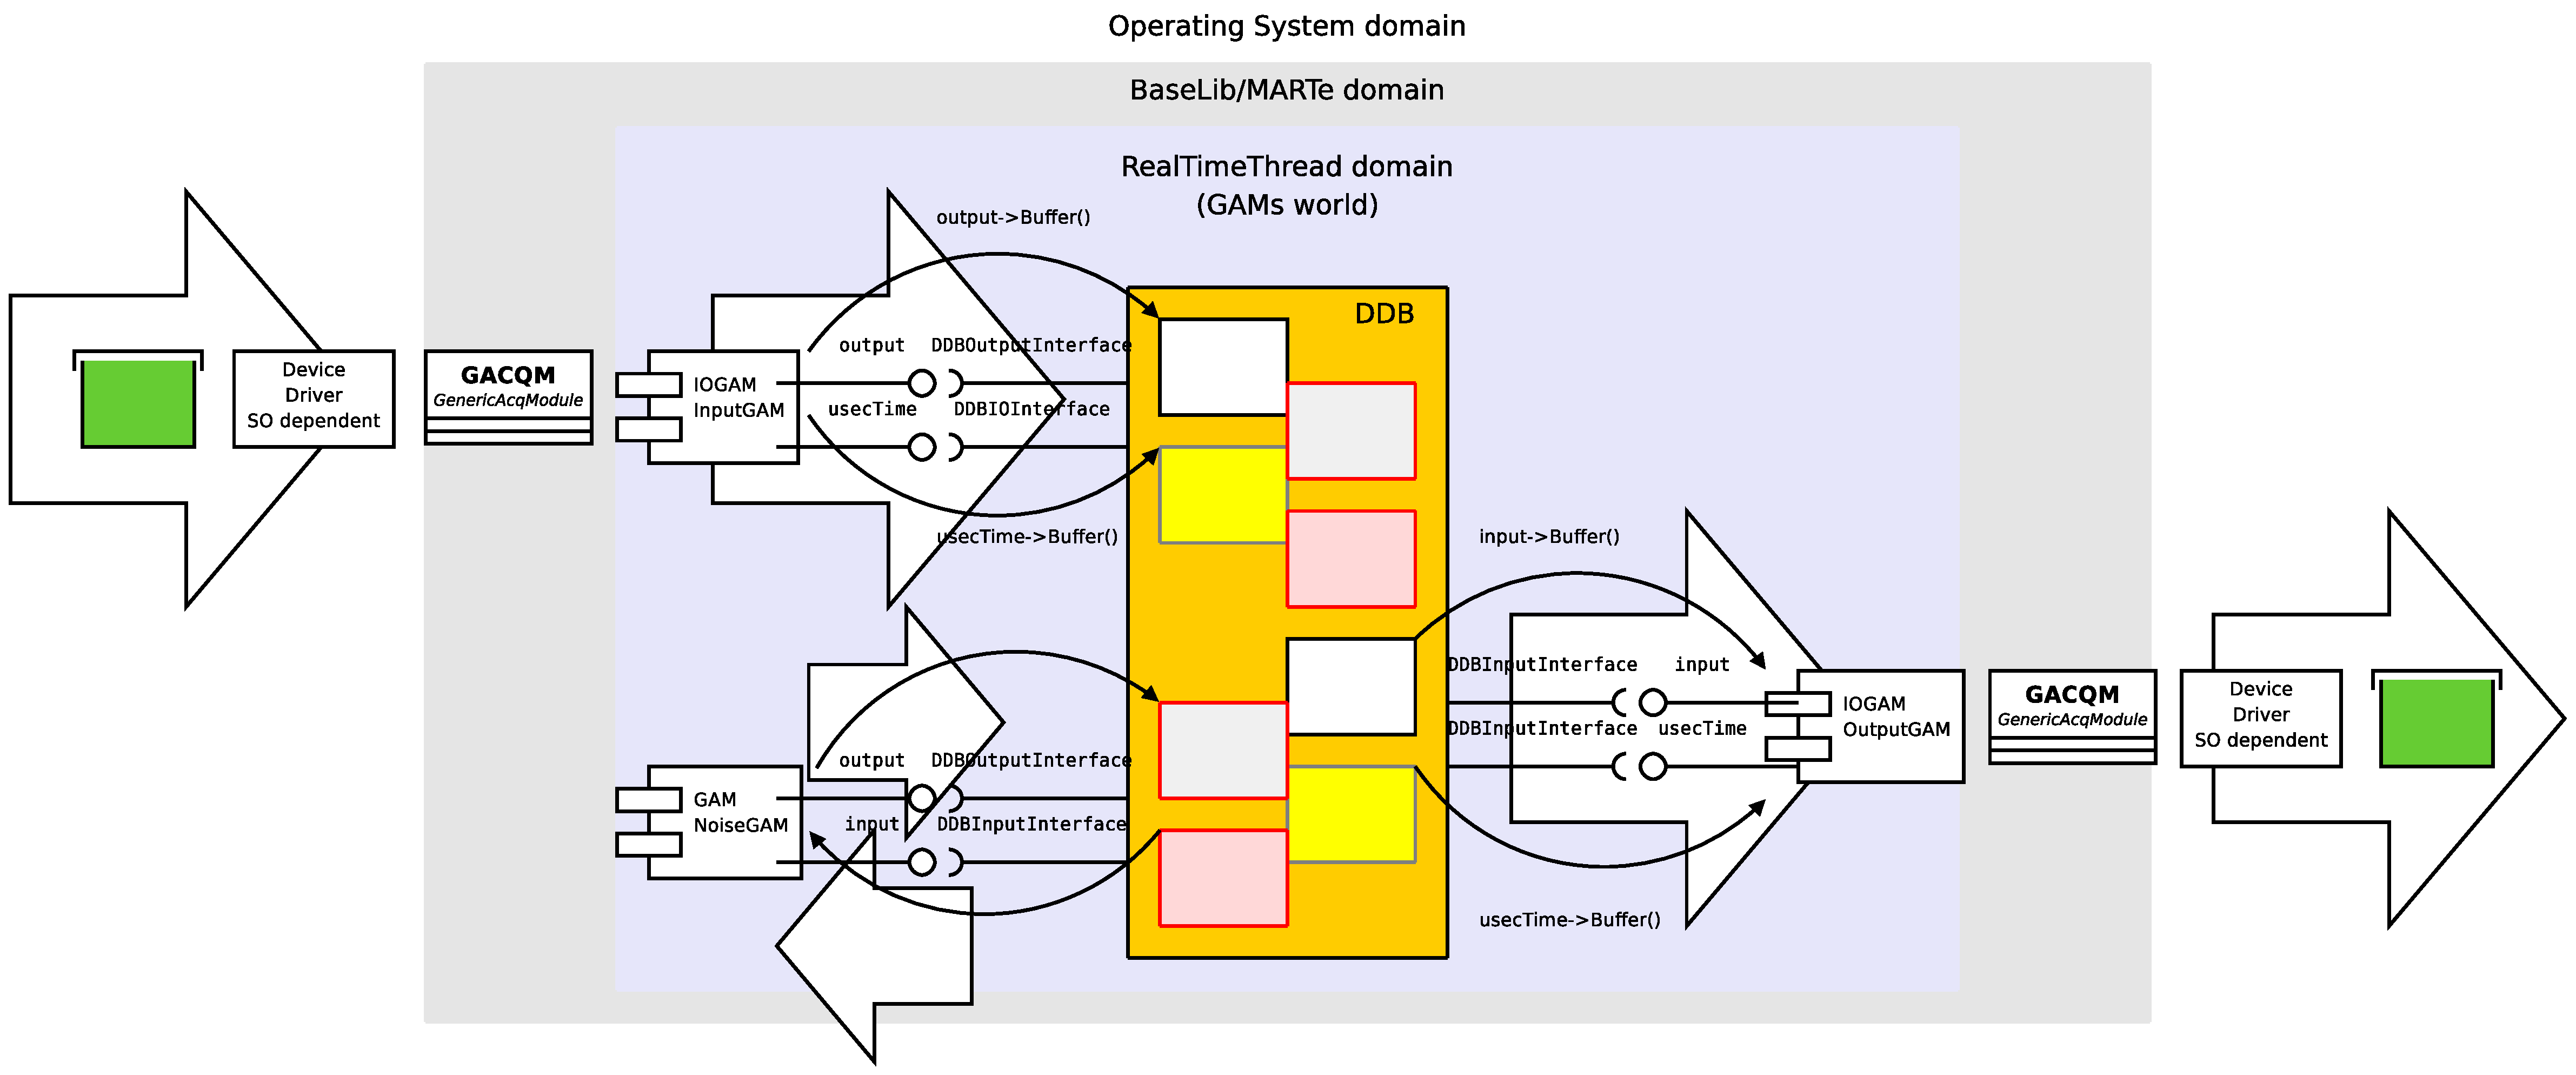
\includegraphics[width=\textwidth]{MARTe/IOGAMs_logic.eps}
  \caption{Different component's domains in MARTe. GAMs (like the \texttt{NoiseGAM} depicted) interact with the system reading and writing on the DDB, obviously they belong to the \textit{GAMs world} like the \texttt{IOGAM}s.}
  \label{f:MARTe:IOGAMs_logic}
 \end{center}
\end{figure}

Using the DDB different GAMs (the basic executing component of the framework) exchange datas. Data on the DDB must be in a predefined format, i.e. all data must be written or read in \texttt{float} or \texttt{int}. Through the chapter different GAMs are presented and not all GAMs agree on the same data format, instead some expect \texttt{float} data and some other \texttt{int} data.\\


This description terminate the whole walk on the components of BaseLib/MARTe validating the component design model adopted during the development of the framework. This kind of component object model design lets start a series of further development to create a simple IDE that helps the user smiply design its control system application and output a configuration that is ready to work in BaseLib/MARTe on the fly.



\section{Input Output Generic Application Modules (IOGAMs)}
This section addresses how a device driver (GACQM) can interact in the GAMs world: it needs a component interface called IOGAM, that infact is a GAM and can be an \texttt{InputGAM} or an \texttt{OutputGAM}. The UML schema in Figure \ref{f:MARTe:IOGAMs} depict the inheritance relationship. Usually an input device can simply act as a counter and infact producing only timing references, some other also data; by the way \texttt{InputGAM}s are specialized in \texttt{TimeInputGAM} that are blocking GAMs that waits for the synchronization from a device driver. \\

\begin{figure}[h!]
 \begin{center}
  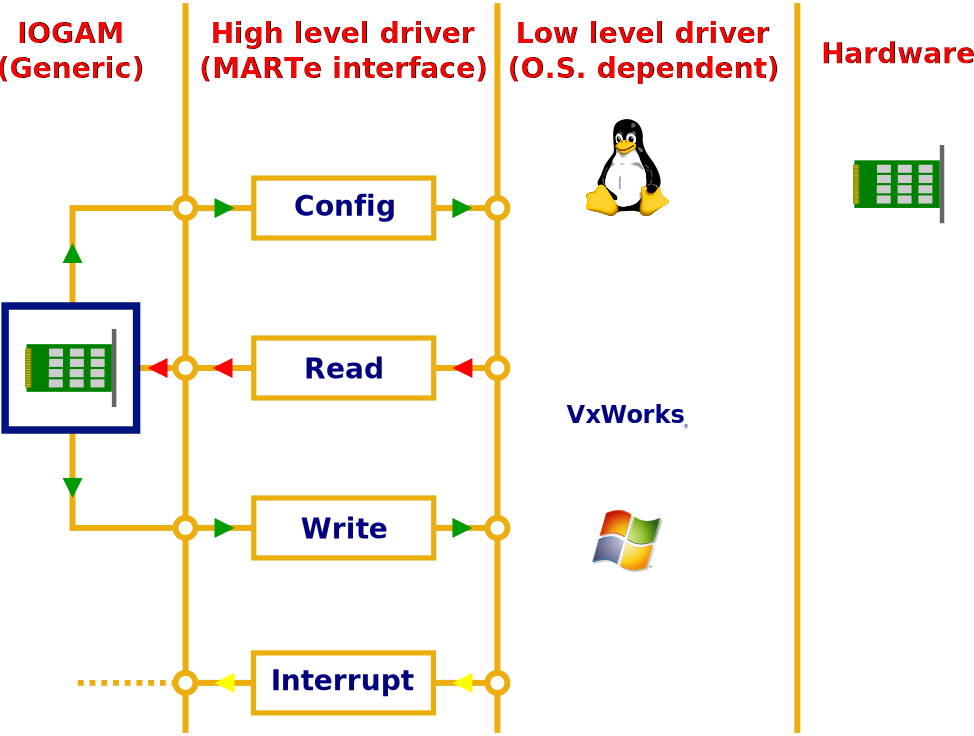
\includegraphics[width=\textwidth]{MARTe/IOGAMs.eps}
  \caption{MARTe Input Output GAMs infrastructure}
  \label{f:MARTe:IOGAMs}
 \end{center}
\end{figure}

Another specializations of the \texttt{InputGAM} are the \texttt{FilteredInputGAM} and the \texttt{TimeFilteredInputGAM}. Those act as median filters on the input signal, if the \texttt{GetData} of the \texttt{GACQM} is synchronized, i.e. is blocking, the \texttt{TimeFilteredInputGAM} decimate the frequency of the input signal. \\

Then follow a list of the involved classes in this section:

\begin{itemize}
 \item InputGAM
 \item TimeInputGAM
 \item FilteredInputGAM
 \item TimeFilteredInputGAM
 \item OutputGAM
\end{itemize}

Figure \ref{f:MARTe:GACQM:IOGAM:Timing} gives a logical understanding of the links between the different component objects (that belongs to different domains) for an acqusition device driver that offer also timing synchronization facilities (in the Figure an \texttt{InterruptDrivenTTS} driver is depicted). Note that a GACQM to produce also timing signals must have a link with a \texttt{TimeInputGAM} not only an \texttt{InputGAM}. The \texttt{TimeInputGAM} by the way must hold a link to GACQM and to the correct \texttt{InterruptDrivenTTS}, i.e. the one that belongs to the same device driver.

\begin{figure}[h!]
 \begin{center}
  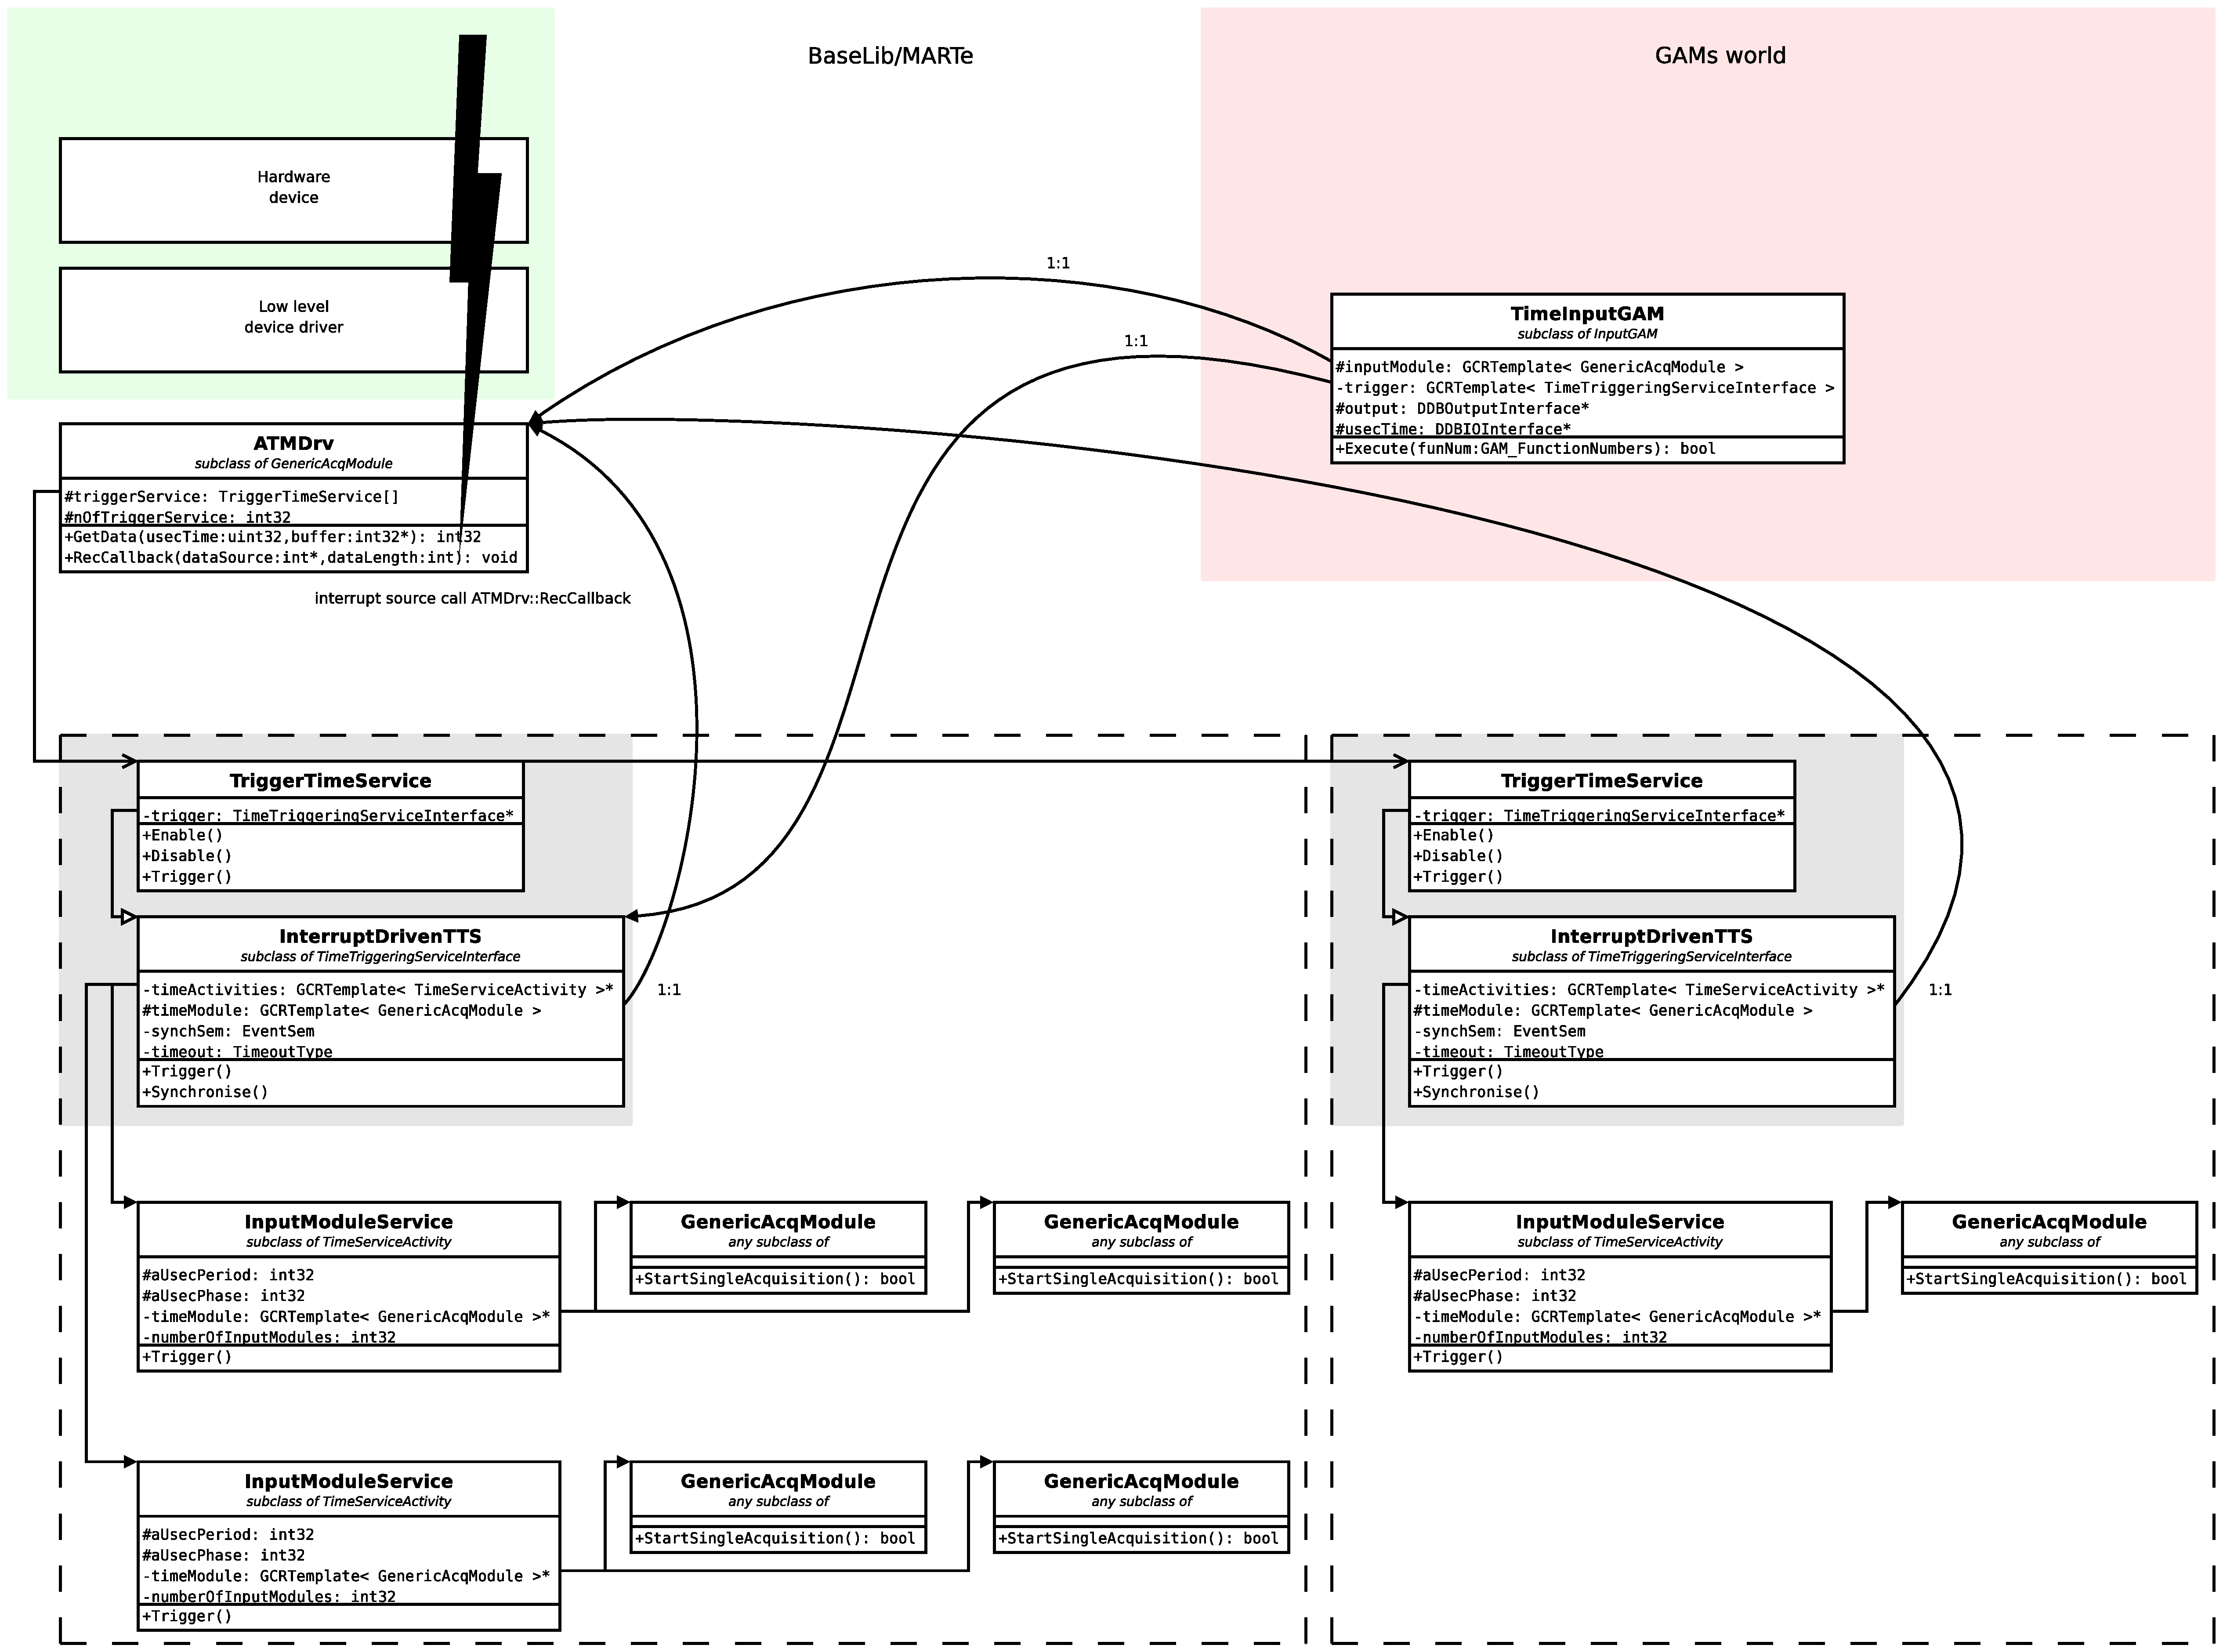
\includegraphics[width=\textwidth]{MARTe/InterruptDrivenTTS_driver.eps}
  \caption{Existent links between a \texttt{GenericAcqModule} a \texttt{TimeInputGAM} and the TTSI infrastructure}
  \label{f:MARTe:GACQM:IOGAM:Timing}
 \end{center}
\end{figure}



\subsubsection{InputGAM}
\texttt{[InputGAM.h, InputGAM.cpp]}\\
The class \texttt{InputGAM} extends \texttt{GAM}, \texttt{HttpInterface} and \texttt{MessageHandler}. The \texttt{InputGAM} is a special GAM that move data, when is ready, from a GACQM  to a memory buffer in the DDB, then the happenning of the event is triggered down to other objects. \\


An \texttt{InputGAM} represent a single device driver that produce input data; the first attribute is infact a \texttt{GCRTemplate} templetized on a \texttt{GenericAcqModule}, i.e. it refers to a single class \texttt{GenericAcqModule}, in other words to one device driver. The attribute \texttt{output} is a pointer to a \texttt{DDBOutputInterface} that is a \texttt{DDBInterface} that has the \texttt{Write} method, thanks to complying to this interface the \texttt{InputGAM} has a buffer where to \textbf{write} in the DDB. This IOGAM has an \texttt{DDBOutputInterface} because looking at the logical block \texttt{InputGAM} it produces data, at the end of the data production (all data has been written to the DDB) the code calls \texttt{DDBOutputInterface::Write()}.

There is another \texttt{DDBInterface} attribute that defines an IO activity, this is \texttt{usecTime}. This attribute is define as an IO interface because a data acquisition board can also write or read a time stamp. The current implementation only read time stamps.

The attribute \texttt{numberOfInputs} is the number of input of the board or also the size of the packet to be readed on the board in words, a word in this case is an \texttt{int32} (see \textit{Level5/DDBInterface.h:BufferSize()}).\\


Then it follows differents calibration factors vector attributes that lets the software convert data from the board data format, \texttt{cal0}, \texttt{oldCal0} and \texttt{cal1}. \texttt{needsCalibration} is an array used to specify if a signal needs calibration. We now have a look on how these variables are used.

The following piece of code is an example from \texttt{InputGAM::Execute(functionNumber=GAMOnline)} about how the previous software calibration variables are used to perform signal value conversion from \texttt{integer} to \texttt{float}. \texttt{cal1[]} is a multiplicative factor and \texttt{cal0[]} is a additive offset.

\begin{lstlisting}[
extendedchars=true,%
basicstyle=\fontfamily{pcr}\fontseries{m}\selectfont\footnotesize, %
stepnumber=1,%
numberstyle=\tiny,%
keywordstyle=\footnotesize\tt ,%
language=C++]
   float* floatBuffer = (float*)output->Buffer();
   int*   intBuffer   = (int*)  output->Buffer();
// ...
   if(inputModule->GetData(time,output->Buffer()) == -1){
      AssertErrorCondition(FatalError,"InputGAM::Execute:: Module %s"
         "GetData Failed for driver %s",Name(),inputModule->Name());
      return False;
   }
   for(int sig=0; sig<numberOfInputs; sig++)
      if(needsCalibration[sig])
         floatBuffer[sig] = (intBuffer[sig]*cal1[sig] + cal0[sig]);
\end{lstlisting}


\textbf{This code imply that the internal data exchange between GAMs can be or in \texttt{integer} or in \texttt{float} data format. If the attribute \texttt{needsCalibration[]} is true values are in \texttt{float} otherwise in \texttt{int}.} \\


All attributes that follow are used to calculate a new calibration value \texttt{cal0} automatically. A first set of \texttt{offsetCompensation} values are computed at startup in \texttt{startUpCycleNumber} iterations, then, during offline \texttt{cal0} factors are updated. The code that follows is executed at 
\texttt{InputGAM::Execute(functionNumber=GAMStartUp)} after the board has read inputs.

\begin{lstlisting}[
extendedchars=true,%
basicstyle=\fontfamily{pcr}\fontseries{m}\selectfont\footnotesize, %
stepnumber=1,%
numberstyle=\tiny,%
keywordstyle=\footnotesize\tt ,%
language=C++]
   if(automaticOffsetCompensation == False) return True;
   startUpCycleNumber++;
   for(int sig = 0; sig < numberOfInputs; sig++){
      if(needsCalibration[sig]) {
         floatBuffer[sig]         = (intBuffer[sig]*cal1[sig] + cal0[sig]);
         offsetCompensation[sig] +=  floatBuffer[sig] - cal0 \begin{center}
  \vspace{0.5cm}
%  \includegraphics[width=30mm]{PPCClogoRed.eps}
  
\includegraphics[width=30mm]{PPCClogoBlack.eps}
 \end{center}[sig]; 
      }
   }
   performOffsetCheck = True;
   if(startUpCycleNumber == offsetCompensationNumberOfCycles)
      calibrationRequested = False;
\end{lstlisting}

The attribute \texttt{automaticOffsetCompensation} enables automatic offset compensation. The attribute \texttt{startUpCycleNumber} is a counter of computed startup cycles in which the \texttt{offsetCompensation} values were updated for each channel. \texttt{offsetCompensation} is a float array where each value is equal to the average of the input signal during offline operations and computed during \texttt{GAMStartUp} phase.

The flag \texttt{performOffsetCheck} marks the transition between \texttt{GAMStartUp} and \texttt{GAMOffline}, at this point the code performs the maximum correction check, if the check fails, the GAM return \texttt{False}, causing the \texttt{RealTimeThread} to perform safety operations. \texttt{offsetCompensationNumberOfCycles} is the number of startup cycles to perform for each calibration. \texttt{calibrationRequested} is a flag set to \texttt{True} when a data calibration is requested. \\


Other attributes are used in the following piece of code, \texttt{InputGAM::Execute(functionNumber=GAMOffline)}:

\begin{lstlisting}[
extendedchars=true,%
basicstyle=\fontfamily{pcr}\fontseries{m}\selectfont\footnotesize, %
stepnumber=1,%
numberstyle=\tiny,%
keywordstyle=\footnotesize\tt ,%
language=C++]
   if(performOffsetCheck){
      for(int sig = 0; sig < numberOfInputs; sig++){
         if((needsCalibration[sig]) && (startUpCycleNumber != 0)){ 
            if(noOffsetAdjustment[sig] == 1) continue;
            offsetCompensation[sig] = offsetCompensation[sig]/startUpCycleNumber;
            cal0[sig] = physicalOffsetValue[sig] - offsetCompensation[sig];
            float offsetPercent = fabs((cal0[sig] - oldCal0[sig])/(cal1[sig]*MAX32BitsValue));
            if(offsetPercent > percentageCorrection){
               AssertErrorCondition(Warning,
                  "InputGAM::Execute:: Module %s: Offset NOT corrected"
                  " %f >allowed %f for driver %s, signal %d, oldcal0 = %e, newcal0=%e",
                  Name(),offsetPercent,percentageCorrection,inputModule->Name(),sig,
                  oldCal0[sig],cal0[sig]);
               cal0[sig] = oldCal0[sig];
            }
         }
      }
      startUpCycleNumber = 0;
      ConfigurationDataBase cdb; ObjectSaveSetup(cdb, NULL); UpdateGAMPersistentCDB(cdb);
      performOffsetCheck = False;
   }
\end{lstlisting}

The attribute \texttt{noOffsetAdjustment} is an array of \texttt{int32} and if not $1$ lets the calibration routine proceed. 

The attribute \texttt{physicalOffsetValue} is an array of defualts offset values for each channel, \texttt{MAX32BitsValue} is the maximum value of a signed 32 bits variable; \texttt{percentageCorrection} is the maximum allowed percentage correction. \\

The last attribute \texttt{currentExecutionState} is the current execution state.
Then the list of all attributes come.

\begin{lstlisting}[
extendedchars=true,%
basicstyle=\fontfamily{pcr}\fontseries{m}\selectfont\footnotesize, %
stepnumber=1,%
numberstyle=\tiny,%
keywordstyle=\footnotesize\tt ,%
language=C++]
protected:  
   GCRTemplate<GenericAcqModule> inputModule;

   DDBOutputInterface* output;
   DDBIOInterface* usecTime;
   int32 numberOfInputs;

   float* cal0;
   float* oldCal0;
   float* cal1;
   bool* needsCalibration;

   bool automaticOffsetCompensation;
   int32* noOffsetAdjustment;
   float* offsetCompensation;
   float* physicalOffsetValue;
   float percentageCorrection;

   static const int32 MAX32BitsValue;
   bool performOffsetCheck;
   bool calibrationRequested;
   int32 startUpCycleNumber;
   int32 offsetCompensationNumberOfCycles;

   GAM_FunctionNumbers currentExecutionState;
\end{lstlisting}

For the first time we have no \texttt{ObjectLoadSetup} method; such method is here substituite by the \texttt{ReadConfigurationFromCDB} method, in this case a \texttt{CDBExtended} is required, not a simpler \texttt{ConfigurationDataBase}. \texttt{ReadConfigurationFromCDB} doesn't suffice and another method \texttt{InitialiseTimeInformation} is necessary to initialise the \texttt{usecTime} \texttt{DDBInterface}. Keep in mind that the \texttt{ObjectLoadSetup} is implemented in the \texttt{GAM} superclass. \\


The method \texttt{ReadTime} reads timing informations, it is only used if the module is a standard \texttt{InputGAM}. The method \texttt{Initialise} initialises the module from a CDB, it uses \texttt{ReadConfigurationFromCDB} and \texttt{InitialiseTimeInformation}; the user must specify the following parameters:
\begin{itemize}
 \item \texttt{BoardName} is the name of the input driver to be used;
 \item \texttt{UsecTimeSignalName} is the name of the time signal in $\mu$sec;
 \item \texttt{Signals} which contains the informations for the ddb interface and the calibrations (if needed);
\end{itemize}

The method \texttt{Execute} executes the module functionalities. The functions or states of a GAM are defined by the enum \texttt{GAM\_FunctionNumbers} in \textit{BaseLib/Level5/GAM.H} an \texttt{InputGAM} implements the following states:
\begin{itemize}
 \item \texttt{GAMStartUp}
 \item \texttt{GAMPrepulse}
 \item \texttt{GAMOffline}
 \item \texttt{GAMOnline}
\end{itemize}

The method \texttt{ObjectSaveSetup} implements the saving of the parameters to a \texttt{ConfigurationDataBase}; \texttt{InputDump} implements the dump of the outputs, with their values, names and calibration factors; \texttt{IsSynchronizing} returns \texttt{True} if the module has delayed acquisition or the associated driver is synchronising.

The method \texttt{ProcessHttpMessage} implements the \texttt{HttpInterface} interface and \texttt{ProcessMessage} implements the \texttt{MessageHandler} interface accepting a message with initialisation requirement.

\begin{lstlisting}[
extendedchars=true,%
basicstyle=\fontfamily{pcr}\fontseries{m}\selectfont\footnotesize, %
stepnumber=1,%
numberstyle=\tiny,%
keywordstyle=\footnotesize\tt ,%
language=C++]
   bool ReadConfigurationFromCDB(CDBExtended& cdb);

   virtual bool InitialiseTimeInformation(ConfigurationDataBase& cdbData);
   virtual int32 ReadTime();

public:
   InputGAM();
   virtual ~InputGAM();

   virtual bool Initialise(ConfigurationDataBase& cdbData);
   virtual bool Execute(GAM_FunctionNumbers functionNumber);

   virtual bool ObjectSaveSetup(ConfigurationDataBase& info, StreamInterface* err);
   bool InputDump(StreamInterface& outputStream);

    virtual bool IsSynchronizing();

    virtual bool ProcessHttpMessage(HttpStream& hStream);
    virtual bool ProcessMessage(GCRTemplate<MessageEnvelope> envelope);
\end{lstlisting}



\subsubsection{FilteredInputGAM}
\texttt{[FilteredInputGAM.h, FilteredInputGAM.cpp]}\\
The class \texttt{FilteredInputGAM} inherits from \texttt{InputGAM} and acts as a medianfilter on \texttt{downsampling} samples of every data source. \\

The core of this class is the \texttt{Execute} method; each \texttt{GAM\_FunctionNumbers} that differ from \texttt{GAMPrepulse} execute the following code:

\begin{lstlisting}[
extendedchars=true,%
basicstyle=\fontfamily{pcr}\fontseries{m}\selectfont\footnotesize, %
stepnumber=1,%
numberstyle=\tiny,%
keywordstyle=\footnotesize\tt ,%
language=C++]
// Reset the OutputInterface
   int sig;
   for(sig=0; sig < output->BufferWordSize(); sig++) floatBuffer[sig]=0.0;
// Copy the data in the buffer and peform filtering activities 
   for(int32 i = 0; i < downSampling; i++ ) {
      if(inputModule->GetData(time,(int32*)buffer,-i) == -1) {
         AssertErrorCondition(FatalError,"InputGAM::Execute:: Module %s GetData Failed"
            " for driver %s", Name(), inputModule->Name());
         return False;
      }
      for(sig=0; sig < output->BufferWordSize(); sig++)
         floatBuffer[sig] += buffer[sig]*filterCoefficients[i];
   }
// Copy last value of integer entries in the DDB
   for(sig = 0; sig < output->BufferWordSize(); sig++) {
      int32 *intB = (int32 *)buffer;
      if(inputModule->GetData(time,(int32 *)buffer,0) == -1) {
         AssertErrorCondition(FatalError,"InputGAM::Execute:: Module %s GetData Failed"
            " for driver %s",Name(), inputModule->Name());
         return False;
      }
      if(needsCalibration[sig])  intBuffer[sig]=intB[sig];
   }
\end{lstlisting}

In such code the \texttt{floatBuffer} array is first filled with zeroes and then each buffer of the circular data buffer of the \texttt{GetData} method of a GACQM is readed, the values in the array are updated with the currently readed ones multiplicate by the \texttt{filterCoefficients[]} factor. The integer \texttt{downSampling} attribute is the frequency divide factor, i.e. every \texttt{downSampling} samples readed from the acquisition board a single event is reported to all the system. Last cycle in the above code seemes to be wrong, probably to be removed.


As we can know from the previous code data are first collected inside the driver, using for example a circular buffer, then copied to the area pointed to the \texttt{buffer} attribute and after some simple calculation saved in the DDB.\\


\textbf{This component assume to has \texttt{float} values as input and \texttt{float} values as output, i.e. the GACQM associated with this GAM must produce \texttt{float} values. This component require that the associated GACQM has a circular buffer of at least \texttt{downSampling} buffers.} \\


All methods that follows behave in the same way as described for the class \texttt{InputGAM}.

\begin{lstlisting}[
extendedchars=true,%
basicstyle=\fontfamily{pcr}\fontseries{m}\selectfont\footnotesize, %
stepnumber=1,%
numberstyle=\tiny,%
keywordstyle=\footnotesize\tt ,%
language=C++]
private:
   float* buffer;
   float* filterCoefficients;
   int32 downSampling;

public:
   FilteredInputGAM();
   virtual ~FilteredInputGAM();

   virtual bool Initialise(ConfigurationDataBase& cdbData);
   virtual bool Execute(GAM_FunctionNumbers functionNumber);

   virtual bool ObjectSaveSetup(ConfigurationDataBase& info,StreamInterface* err);
   virtual bool IsSynchronizing();
\end{lstlisting}



\subsubsection{TimeFilteredInputGAM}
\texttt{[TimeFilteredInputGAM.h, TimeFilteredInputGAM.cpp]}\\
A \texttt{TimeFilteredInputGAM} class inherits from \texttt{FilteredInputGAM} adding a reference to a triggering service facility (\texttt{GCRTemplate<TimeTriggeringServiceInterface>}).
This timing triggering service facility is used in the \texttt{Execute} method that basically call the same method of the superclass first waiting on the \texttt{Synchronise} method of the attribute added.

\begin{lstlisting}[
extendedchars=true,%
basicstyle=\fontfamily{pcr}\fontseries{m}\selectfont\footnotesize, %
stepnumber=1,%
numberstyle=\tiny,%
keywordstyle=\footnotesize\tt ,%
language=C++]
private:
   GCRTemplate<TimeTriggeringServiceInterface> trigger;

   virtual bool InitialiseTimeInformation(ConfigurationDataBase& cdbData);
   virtual int32 ReadTime();

public:
   TimeFilteredInputGAM();
   virtual ~TimeFilteredInputGAM();

   virtual bool Initialise(ConfigurationDataBase& cdbData);
   virtual bool Execute(GAM_FunctionNumbers functionNumber);

   virtual bool ObjectSaveSetup(ConfigurationDataBase& info,StreamInterface* err);
   bool InputDump(StreamInterface& outputStream);
   virtual bool IsSynchronizing();
\end{lstlisting}



\subsubsection{TimeInputGAM}
\texttt{[TimeInputGAM.h, TimeInputGAM.cpp]}\\
A \texttt{TimeInputGAM} as a \texttt{TimeFilteredInputGAM} does on a \texttt{FilteredInputGAM} adds a reference to a triggering service facility to the \texttt{InputGAM} class from which it inherits.

The only thing that changes, compared to the \texttt{InputGAM} class, is that on the \texttt{Execute} method before calling the superclass's one the \texttt{TimeTriggeringServiceInterface::Synchronise} method is called.

\begin{lstlisting}[
extendedchars=true,%
basicstyle=\fontfamily{pcr}\fontseries{m}\selectfont\footnotesize, %
stepnumber=1,%
numberstyle=\tiny,%
keywordstyle=\footnotesize\tt ,%
language=C++]
private:
   GCRTemplate<TimeTriggeringServiceInterface> trigger;

   virtual bool InitialiseTimeInformation(ConfigurationDataBase& cdbData);
   virtual int32 ReadTime();

public:
   TimeInputGAM();
   virtual ~TimeInputGAM();

   virtual bool Initialise(ConfigurationDataBase& cdbData);
   virtual bool Execute(GAM_FunctionNumbers functionNumber);

   virtual bool ObjectSaveSetup(ConfigurationDataBase& info,StreamInterface* err);
   bool InputDump(StreamInterface& outputStream);

   virtual bool IsSynchronizing();
\end{lstlisting}



\subsubsection{OutputGAM}
\texttt{[OutputGAM.h, OutputGAM.cpp]}\\
The class \texttt{OuputGAM} extends \texttt{GAM}; \texttt{OutputGAM} is a special GAM that move data, when is executed, from a memory buffer in the DDB to a GACQM. \\


An \texttt{OutputGAM} represent a single device driver that output data; the first attribute is infact a \texttt{GCRTemplate} templetized on a \texttt{GenericAcqModule}, i.e. it refers to a single class \texttt{GenericAcqModule}, in other words to one device driver. The attribute \texttt{input} is a pointer to a \texttt{DDBInputInterface} that is a \texttt{DDBInterface} that has the \texttt{Read} method, thanks to complying to this interface the \texttt{OutputGAM} has a buffer where to \textbf{read} in the DDB. This IOGAM has an \texttt{DDBInputInterface} because looking at the logical block \texttt{OutputGAM} it consumes data, at the start of the data consumation (all data has to be readed to the DDB) the code calls \texttt{DDBInputInterface::Read()} that request valid data on the buffer to the DDB.

There is another \texttt{DDBInterface} attribute that defines another input activity, this is \texttt{usecTime}. This attribute is define as input interface because an output board can only read time stamps.

The attribute \texttt{dataWordSize} is the number of output of the word or also the size of packet to be written on the board in words, a word in this case is an \texttt{int32} (see \textit{Level5/DDBInterface.h:BufferSize()}).\\


Then it follows differents calibration factors vector attributes that lets the software convert data to the board data format, \texttt{cal0}, \texttt{cal1}, \texttt{maxOutputValue} and \texttt{minOutputValue}. \texttt{needsCalibration} is an array used to specify if a signal needs calibration/conversion. The following piece of code is an example from \texttt{OutputGAM::Execute()} about how the previous software calibration variables are used to perform signal value conversion from \texttt{float} to \texttt{integer}. \texttt{cal1[]} is a multiplicative factor and \texttt{cal0[]} is a additive offset.

\begin{lstlisting}[
extendedchars=true,%
basicstyle=\fontfamily{pcr}\fontseries{m}\selectfont\footnotesize, %
stepnumber=1,%
numberstyle=\tiny,%
keywordstyle=\footnotesize\tt ,%
language=C++]
   for(int sig=0; sig < dataWordSize; sig++)
      if(needsCalibration[sig]) {
         float output = floatBuffer[sig];
         if(output > maxOutputValue[sig]) output=maxOutputValue[sig];
         if(output < minOutputValue[sig]) output=minOutputValue[sig];
         float temp  = (output - cal0[sig])*cal1[sig];
         int tempInt = FastFloat2Int(temp);
         intBuffer[sig] = tempInt;
      }
\end{lstlisting}

Obviously the attribute \texttt{maxOutputValue} is the maximum output value and \texttt{minOutputValue} is the minimum output value; \texttt{cal0} and \texttt{cal1} has the same meaning as in the \texttt{InputGAM} module.

\begin{lstlisting}[
extendedchars=true,%
basicstyle=\fontfamily{pcr}\fontseries{m}\selectfont\footnotesize, %
stepnumber=1,%
numberstyle=\tiny,%
keywordstyle=\footnotesize\tt ,%
language=C++]
private:
   GCRTemplate<GenericAcqModule> outputModule;

   DDBInputInterface* input;
   DDBInputInterface* usecTime;
   int32 dataWordSize;

   float* cal0;
   float* cal1;
   float* maxOutputValue;
   float* minOutputValue;
   bool* needsCalibration;
\end{lstlisting}

The method \texttt{Initialise} initialises the IOGAM reading the configuration from a CDB; \texttt{Execute} executes the data transfer from memory in the DDB to the GACQM, the only implemented \texttt{GAM\_FunctionNumbers} states are: \texttt{GAMOffline} and \texttt{GAMOnline}.

\begin{lstlisting}[
extendedchars=true,%
basicstyle=\fontfamily{pcr}\fontseries{m}\selectfont\footnotesize, %
stepnumber=1,%
numberstyle=\tiny,%
keywordstyle=\footnotesize\tt ,%
language=C++]
public:
   OutputGAM();
   virtual ~OutputGAM();

   virtual bool Initialise(ConfigurationDataBase& cdbData);
   virtual bool Execute(GAM_FunctionNumbers functionNumber);

   virtual bool ObjectSaveSetup(ConfigurationDataBase& info,StreamInterface* err);

   bool OutputDump(StreamInterface& outputStream);
   virtual bool IsSynchronizing();
\end{lstlisting}



\subsection{Design Notes}
In MARTe the directory \textit{MARTe/IOGAMs} contains a set of classes that are to compiled in a unique sub library of the framework, the library in a UNIX system has the name \textit{libIOGAM.so}. By the way exist the file \texttt{IOGAM.cpp} and is empty, this file is needed to generate \textit{libIOGAM.so} and makes the compiler happy. \\


Some more words about the IOGAMs. The difference between an \texttt{InputGAM} and a \texttt{TimeInputGAM} is basically in the \texttt{Execute} method, moreover a \texttt{TimeInputGAM} has a reference to a \texttt{TimeTriggeringServiceInterface}. Such interface lets the \texttt{TimeInputGAM} call its \texttt{Synchronise} method before executing the normal \texttt{Execute} method of the GAM. \\


How an IOGAM works depends heavily on how a GACQM is implemented. The most important method regarding our discussion is the \texttt{GetData}. The \texttt{GetData} method must be non blocking letting a caller read an internal data buffer. Some implementation, like the ATMDrv (that we will see in the next section), lets the user deciding if the \texttt{GetData} must be blocking or non blocking. Such solution probably is not the best one possible because can confuse if seen at high level.
For example it change completely how a \texttt{FilteredInputGAM} works; but also change the way in which a \texttt{TimeInputGAM} react. Thinking about the simplest case, i.e. the \texttt{TimeInputGAM}, on \texttt{Execute} it calls \texttt{InterruptDrivenTTS::Synchronise} that waits for interrupt, then it calls \texttt{GenericAcqModule::GetData} that is blocking and waits from another interrupt dividing the frequency of data arrivals. Keep in mind that if you have a synchronising \texttt{GetData} your synchronising method must always return \texttt{True}. A stronger design must be applied. Something similar happens with the \texttt{FilteredInputGAM} and the \texttt{TimeFilteredInputGAM}. Furthermore such classes act as a downsampler not as a median filter. \\


The following code require a double discussion. First of all is notable that the same area of memory can be handled as a float array or as a integer array, consistency about type casting aslo at runtime is compulsatory.

A second notes is about performance and efficiency last two code lines can be executed by FPU optimized SIMD instructions. Think about the Altivec unit, it has one single assemply instruction that operates on the same data the instruction is the \textit{Multiply and Add}. Other processor have its own SIMD instruction that must be exploited by our code. Note that SIMD instruction are nowadays a common requirement of all brand new processors also for home user computers. \\

\begin{lstlisting}[
extendedchars=true,%
basicstyle=\fontfamily{pcr}\fontseries{m}\selectfont\footnotesize, %
stepnumber=1,%
numberstyle=\tiny,%
keywordstyle=\footnotesize\tt ,%
language=C++]
   float* floatBuffer = (float*)output->Buffer();
   int*   intBuffer   = (int*)  output->Buffer();

// ...

   for(int sig=0; sig<numberOfInputs; sig++)
      if(needsCalibration[sig])
         floatBuffer[sig] = (intBuffer[sig]*cal1[sig] + cal0[sig]);
\end{lstlisting}



%-----------------------------------------------------------------------------%
%-----------------------------------------------------------------------------%
%-----------------------------------------------------------------------------%



\section{Generic Acquisition Modules (GACQM)}
In this section we are going to analyse the directories contained in the directory \textit{MARTe/IOGAMS}. Note that sources contained in such directory are just been commented in the previous section. Directories we analyse here contain a device driver (GACQM) each. In this section we are going to speak about device drivers, i.e. \texttt{GenericAcqModule}s. Figure \ref{f:MARTe:IOGAMs_Drv} is the UML class diagram of each device driver class object existent in the previous cited directory. \\

\begin{figure}[h!]
 \begin{center}
  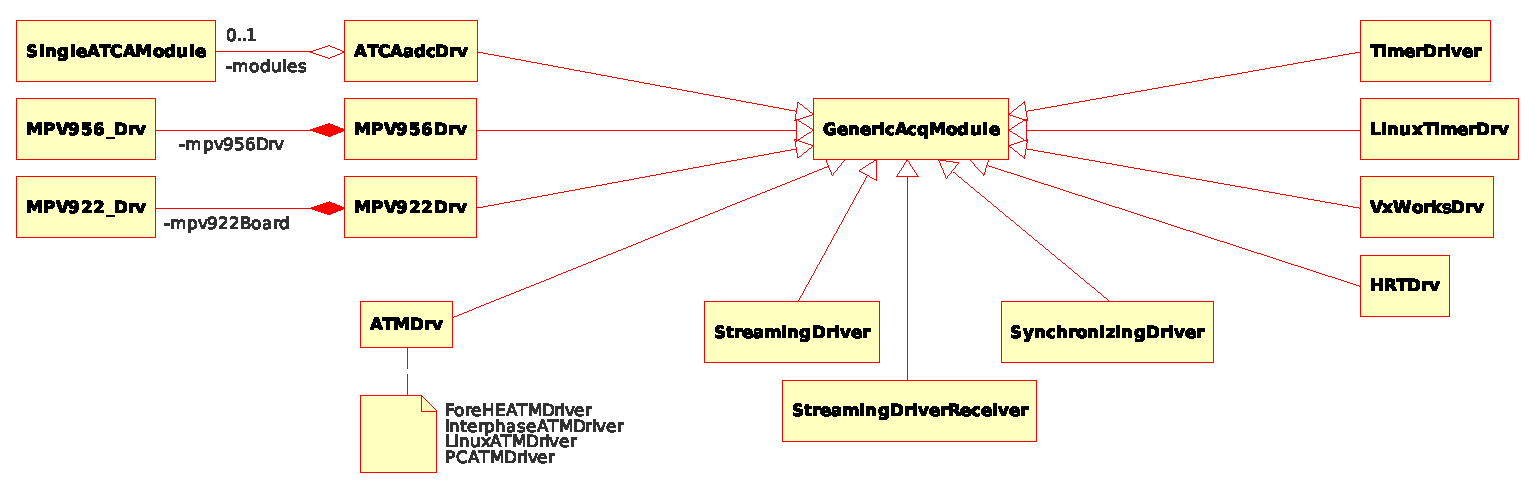
\includegraphics[width=\textwidth]{MARTe/IOGAMs-Drv.eps}
  \caption{MARTe \texttt{GACQM}s }
  \label{f:MARTe:IOGAMs_Drv}
 \end{center}
\end{figure}

We are not going to analyse all device drivers in the library because each device driver is application specific and is not interesting in general. We just focus our attention to two different type of device driver's sychronization. A GACQM that synchronise itself via a \texttt{InterruptDrivenTTS} interface (\texttt{ATMDrv}) and a GACQM that synchronise itself via a \texttt{DataPollingDrivenTTS} interface (\texttt{ATCAadcDrv}). \\

\begin{figure}[h!]
 \begin{center}
  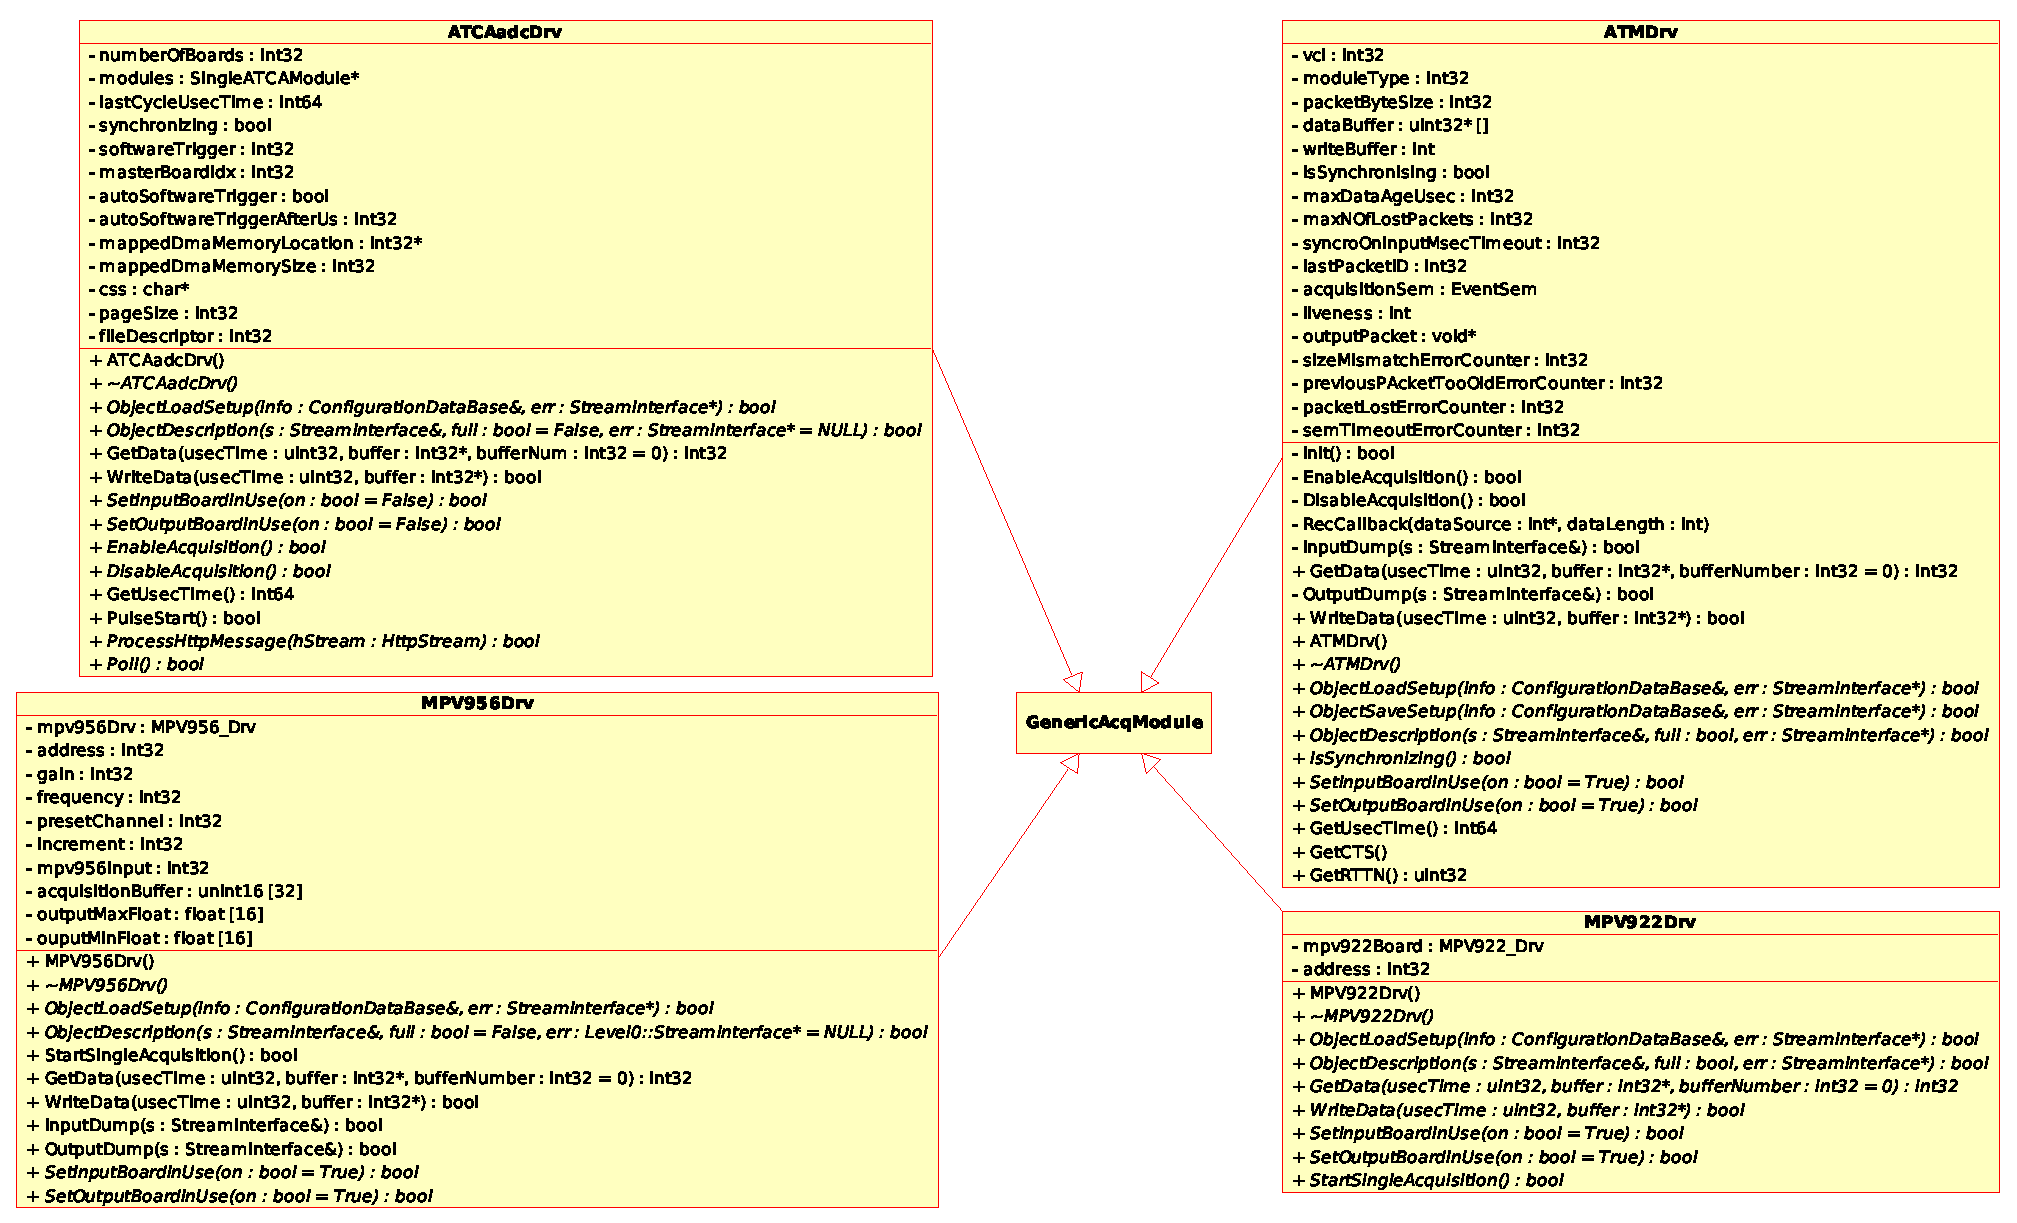
\includegraphics[width=0.93\textwidth]{MARTe/IOGAMs-Drv-Acq.eps}
  \caption{MARTe's hardware \texttt{GACQM}s}
  \label{f:MARTe:IOGAMs_Acq}
 \end{center}
\end{figure}

In Figure \ref{f:MARTe:IOGAMs_Acq} there is the UML class diagram of such GACQMs. Note that between different implementation of the \texttt{GenericAcqModule} class there are just little differences. \\



\subsection{InterruptDrivenTTS GACQM (ATMDrv)}
A \texttt{GenericAcqModule} has as an attribute, an array of \texttt{TriggerTimeService} each of that can hold an implementation of \texttt{TimeTriggeringServiceInterface}. Let's start with the case of a GACQM holding at least one \texttt{InterruptDrivenTTS}. Let's also assume that our device driver generate interrupts on data arrival. What happens on the \texttt{TimeInputGAM} side when executed by the \texttt{RealTimeThread}? We are assuming that the \texttt{GenericAcqModule::GetData} is not blocking, i.e. the module is not synchronising. In Figure \ref{f:MARTe:GACQM:InterruptDrivenTTS} the UML sequence diagram show the method calling sequence.

\begin{figure}[h!]
 \begin{center}
  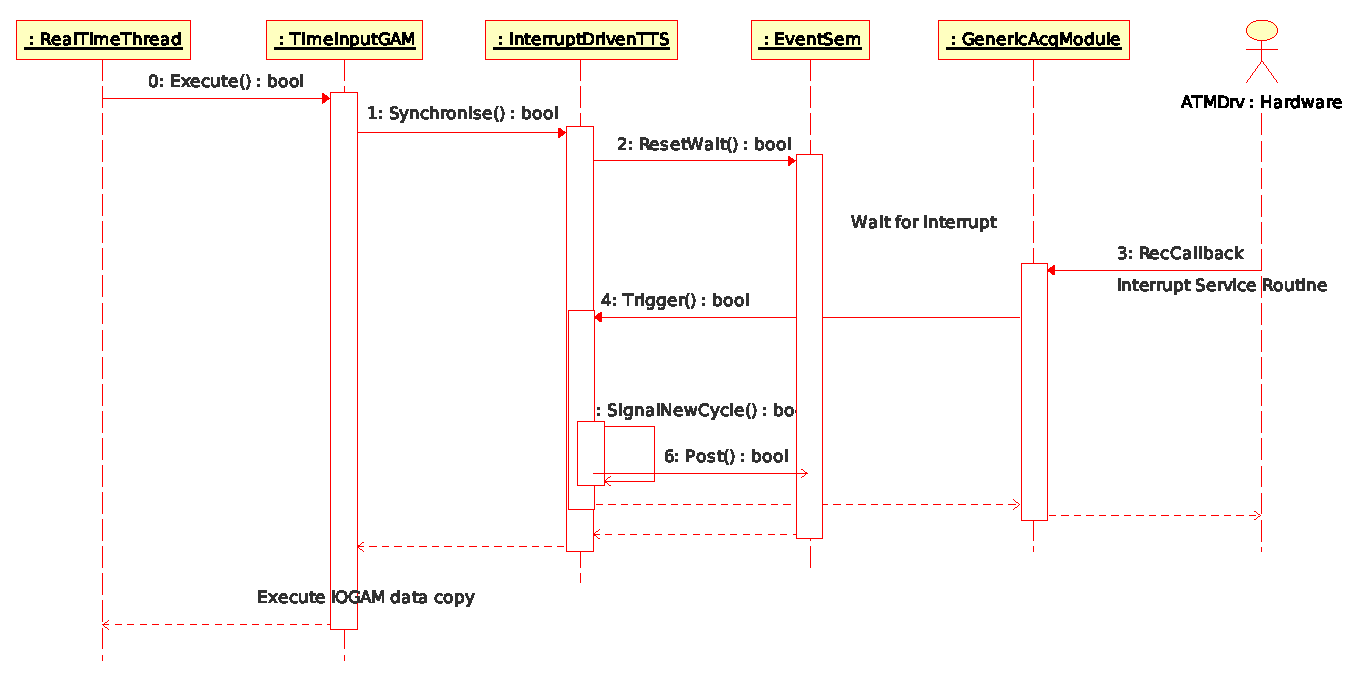
\includegraphics[width=\textwidth]{MARTe/InterruptDrivenTTS.eps}
  \caption{MARTe UML sequence diagram of an \texttt{InterruptDrivenTTS} compatible \texttt{GenericAcqModule} }
  \label{f:MARTe:GACQM:InterruptDrivenTTS}
 \end{center}
\end{figure}

We try to illustrate what happens in the schema in Figure \ref{f:MARTe:GACQM:InterruptDrivenTTS} step by step in the following:

\begin{enumerate}
 \item[0.] the \texttt{RealTimeThread} calls \texttt{TimeInputGAM::Execute} method;
 \item \texttt{TimeInputGAM::Execute} as first action calls \texttt{InterruptDrivenTTS::Synchronise} method;
 \item this method simply calls \texttt{EventSem::ResetWait} method that pauses the \texttt{RealTimeThread} giving the control of the CPU to the operating system that virtually can execute another process.
 \item the device generate an interrupt, i.e. some data is ready to transfer to the main memory (or the transfer is just finished), the associated ISR is called (\texttt{GenericAcqModule::RecCallback};
 \item \texttt{GenericAcqModule::RecCallback} as the last instruction calls method \texttt{Trigger} of all its registered \texttt{TimeTriggeringServiceInterface};
 \item the method \texttt{InterruptDrivenTTS::Trigger} as its last instruction calls \texttt{SignalNewCycle};
 \item the only action that performs \texttt{SingnalNewCycle} is to call \texttt{EventSem.Post} that wakeup the \texttt{RealTimeThread} that can continue its execution exiting from \texttt{InterruptDrivenTTS::Synchronise} and copying the data to the DDB (calling \texttt{GenericAcqModule::GetData} from the \texttt{TimeInputGAM} that is not blocking.
\end{enumerate}

Follows the usual class analysis of the implementing driver, we have to punctualise that the previous described behaviour must only be achieved without a blocking \texttt{GenericAcqModule::GetData} method.

The following \texttt{ATMDrv} can be associated with an \texttt{InputGAM} but also with a \texttt{OutputGAM} because can receive and transmit data.



\subsubsection{ATMDrv}
\texttt{[ATMDrv.h, ATMDrv.cpp]}\\
The code that follow is specifically from the \textit{ForeHEATMDriver} directory; all other ATM driver implementations have a similar high level driver that interface to the BaseLib/MARTe. \\


The class \texttt{ATMDrv} inherits only from \texttt{GenericAcqModule}. An ATM network board is not very common today but permits deterministic transmission times exploiting QoS techiniques both on the trasmitter/receiver side and on the switches of the network. The first attribute, \texttt{vci} is the virtual channel identifier number of the ATM network channel associatedwith the class instance. \texttt{moduleType} identifies if the instance of the module behave as an output or as an input, it can also be undefined if is not just setted. The attribute \texttt{packetByteSize} is the input/output buffer size in byte. \\


The following attributes are used by a receiver channel. \texttt{dataBuffer} is a triple buffer for receiving data, \texttt{nOfDataBuffers} is defined as $3$ in the source code; the class's code allocate three data buffer of size \texttt{packetByteSize} and saves its addresses in the \texttt{dataBuffer} array. \texttt{writeBuffer} is the index of the write only buffer, i.e. the index of the buffer that will be written by the next interrupt data transfer ISR. The attribute \texttt{isSynchronising} specifies if the receiver module is synchornizing or get the latest fullfilled buffer.

The attribute \texttt{maxDataAgeUsec} it is used to decided if the read data are ready or not; \texttt{maxNOfLostPackets} is the maximum number of lost packets after a rollover; \texttt{syncroOnInputMsecTimeout} is the timeout in $msec$ to wait on a synchronization event; \texttt{lastPacketID} is the ID of the last packet received.

The attribute \texttt{acquisitionSem} is an event semaphore to be used in case of a synchornization acquisition mode, i.e. a blocking \texttt{GetData}. The attribute \texttt{liveness} get the liveness of the driver. \\


The attribute \texttt{outputPacket} is a pointer to the actual packet to be sent. It's the only attribute associated to a transmitter module. \\


Finally follows a series of counter attributes, used in transmitter and receiver modules; \texttt{sizeMismatchErrorCounter} counts the number of size mismatch events; reset it as soon as the first correct packet is received. \texttt{previousPacketTooOldErrorCounter} counts the number of packet that was too old; it has to be resetted as soon as the first correct packet is received. \texttt{packetLostErrorCounter} counts the number of lost packets; it is resetted as soon as the first correct packet is received; \texttt{semTimeoutErrorCounter} counts the number of \texttt{EventSem} happens timeouts.

\begin{lstlisting}[
extendedchars=true,%
basicstyle=\fontfamily{pcr}\fontseries{m}\selectfont\footnotesize, %
stepnumber=1,%
numberstyle=\tiny,%
keywordstyle=\footnotesize\tt ,%
language=C++]
private:
   int32 vci;
   int32 moduleType;
   int32 packetByteSize;

   uint32* dataBuffer[nOfDataBuffers];
   int writeBuffer;
   bool isSynchronising;

   int32 maxDataAgeUsec;
   int32 maxNOfLostPackets;
   int32 syncroOnInputMsecTimeout;
   int32 lastPacketID;
   EventSem acquisitionSem;
   int liveness;

   void* outputPacket;

   int32 sizeMismatchErrorCounter;
   int32 previousPacketTooOldErrorCounter;
   int32 packetLostErrorCounter;
   int32 semTimeoutErrorCounter;
\end{lstlisting}

Now we switch to methods of the \texttt{ATMDrv} class. The \texttt{Init} method inits all module entries. \texttt{EnableAcquisition} and \texttt{DisableAcquisition} enables and disables board data acquisition.
The method \texttt{RecCallback} is called from the ISR when the board generate interrupts for data transfer from the board to the main memory. 

\texttt{InputDump} dumps input data to the passed by argument stream; \texttt{GetData} copies data from the device driver to the DDB. \texttt{OutputDump} dumps output data to the passed by argument stream; \texttt{WriteData} copies data from the DDB to the ATM board memory and command a send action to the hardware.\\


The method \texttt{IsSynchronizing} return the value of the attribute \texttt{isSynchronising}. \texttt{SetInputBoardInUse} set the board as an input module an that is in use. The same thing is done from the \texttt{SetOutputBoardInUse} setting the in use state on output. 

\texttt{GetUsecTime} return the time of the last acquistion event, the last two methods, \texttt{GetCTS} and \texttt{GetRTTN} are old and plant (JET) specific and must be removed.

\begin{lstlisting}[
extendedchars=true,%
basicstyle=\fontfamily{pcr}\fontseries{m}\selectfont\footnotesize, %
stepnumber=1,%
numberstyle=\tiny,%
keywordstyle=\footnotesize\tt ,%
language=C++]
private:
   bool Init();

   bool EnableAcquisition();
   bool DisableAcquisition();

   void RecCallback(int* dataSource,int dataLength);
   bool InputDump(StreamInterface& s) const;

public:
   int32 GetData(uint32 usecTime,int32* buffer,int32 bufferNumber=0);

private:
   bool OutputDump(StreamInterface& s)const;

public:
   bool WriteData(uint32 usecTime,const int32* buffer);

private:
   ATMDrv(const ATMDrv& atm);
   ATMDrv& operator=(const ATMDrv& atm);
public:
   ATMDrv();
   ~ATMDrv();

   virtual bool ObjectLoadSetup(ConfigurationDataBase& info,StreamInterface* err);
   virtual bool ObjectSaveSetup(ConfigurationDataBase& info,StreamInterface* err);
   virtual bool ObjectDescription(StreamInterface& s,bool full,StreamInterface* err);

   virtual bool IsSynchronizing();
   virtual bool SetInputBoardInUse(bool on = True);
   virtual bool SetOutputBoardInUse(bool on = True);

   int64 GetUsecTime();
   uint16 GetCTS();
   uint32 GetRTTN();
\end{lstlisting}



\subsection{DataPollingDrivenTTS GACQM (ATCAadcDrv)}
As said in the previous subsection a \texttt{GenericAcqModule} has as an attribute, an array of \texttt{TriggerTimeService} each of that can hold an implementation of \texttt{TimeTriggeringServiceInterface}. In this subsection we analyse the case of a GACQM holding at least one \texttt{DataPollingDrivenTTS}.
What happens on the \texttt{TimeInputGAM} side when executed by the \texttt{RealTimeThread}? We are assuming that the \texttt{GenericAcqModule::GetData} is not blocking, i.e. the module is not synchronising. In Figure \ref{f:MARTe:GACQM:DataPollingDrivenTTS} the UML sequence diagram show the method calling sequence.

\begin{figure}[h!]
 \begin{center}
  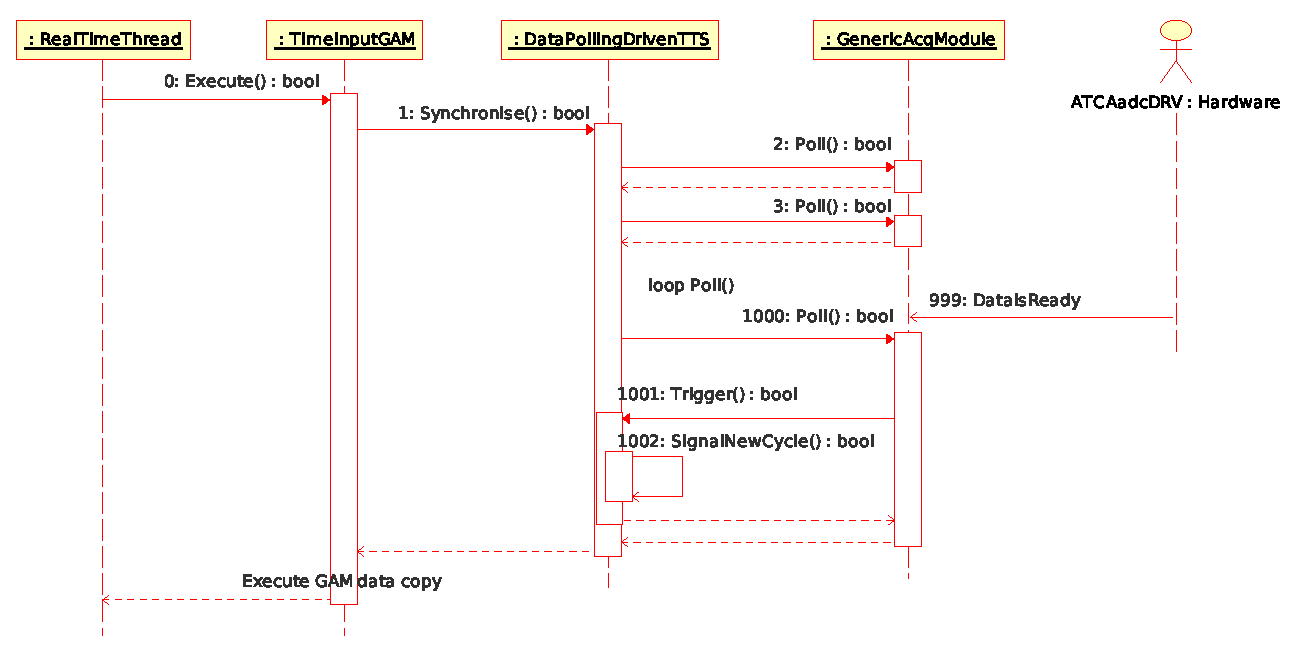
\includegraphics[width=\textwidth]{MARTe/DataPollingDrivenTTS.eps}
  \caption{MARTe UML sequence diagram of a \texttt{DataPollingDrivenTTS} compatible \texttt{GenericAcqModule}}
  \label{f:MARTe:GACQM:DataPollingDrivenTTS}
 \end{center}
\end{figure}

We try to illustrate what happens in the schema in Figure \ref{f:MARTe:GACQM:DataPollingDrivenTTS} step by step in the following:

\begin{enumerate}
 \item[0.] the \texttt{RealTimeThread} calls \texttt{TimeInputGAM::Execute} method;
 \item \texttt{TimeInputGAM::Execute} as first action calls \texttt{DataPollingDrivenTTS::Synchronise} method;
 \item this method implements a loop in which in each iteration \texttt{GenericAcqModule::Poll} is called, if returns \texttt{False} the loop continue;

 \item[999.] the device acquires some data and moves them to the main memory;
 \item[1000.] we are still in the loop in the \texttt{DataPollingDriver::Synchronise} method, a new call to \texttt{Poll} happens;
 \item[1001.] the method \texttt{GenericAcqModule::Poll} identifies that new data is just arrived then calls the \texttt{DataPollingDrivenTTS::Trigger} method;
 \item[1002.] \texttt{DataPollingDrivenTTS::Trigger} as its last instruction calls \texttt{SignalNewCycle};
 \item[1003.] the method \texttt{DataPollingDrivenTTS::SignalNewCycle} modifies an internal variable of the \texttt{DataPollingDrivenTTS} class that lets the \texttt{Synchronise} method exit from the loop and returno control to the \texttt{TimeInputGAM}; as the same time the \texttt{Poll} method return \texttt{True} letting the loop exit in any case. Then follow the data copy activity carried on by code implemented in the \texttt{InputGAM}.
\end{enumerate}

Follows the usual class analysis of the implementing driver.



\subsubsection{ATCAadcDrv}
\texttt{[ATCAadcDrv.h, ATCAadcDrv.cpp]}\\
The class \texttt{ATCAadcDrv} is the high level driver for the ATCA ADC module, an hardward board developed from the JET plant; the class inherits exclusively from \texttt{GenericAcqModule}. \\


The first attribute \texttt{numberOfBoards} is the number of boards in the crate; readed during the initialisation; for each board the class has to create a new instance of the \texttt{SingleATCAModule} class, at the initialization an array of \texttt{SingleATVAModule}s is created and the pointer is holded by the \texttt{modules} attribute. \texttt{masterBoardIdx} is the index of the master board in the crate. \\


The attribute \texttt{lastCycleUsecTime} holds the last cycle time in $\mu$sec; \texttt{synchronizing} is \texttt{True} if the module is synchronizing, i.e. the \texttt{GetData} is blocking. \\


The attribute \texttt{softwareTrigger} configure the board for software triggered acquisition; if the attribute \texttt{autoSoftwareTrigger} is set to true then a software trigger will be sent every \texttt{autoSoftwareTriggerAfterUs} $\mu$sec. This mechanism works if the the value of \texttt{autoSoftwareTriggerAfterUs} in the configuration file is greater then $1$.

Last attribute, \texttt{css} is the pointer to a string that holds the CSS file for the reflection HTTP page. \\

\begin{lstlisting}[
extendedchars=true,%
basicstyle=\fontfamily{pcr}\fontseries{m}\selectfont\footnotesize, %
stepnumber=1,%
numberstyle=\tiny,%
keywordstyle=\footnotesize\tt ,%
language=C++]
private:
   int32 numberOfBoards;
   SingleATCAModule* modules;
   int32 masterBoardIdx;

   int64 lastCycleUsecTime;
   bool synchronizing;

   int32 softwareTrigger;
   bool autoSoftwareTrigger;
   int32 autoSoftwareTriggerAfterUs;

   const char *css;
\end{lstlisting}

The method \texttt{GetData} copies data from the ATCA board into the DDB; \texttt{WriteData} moves data from the DDB to the ATCA board. Note that as the \texttt{ATMDrv} also this class can act as input and as output. \\

The method \texttt{PulseStart} is used for simulation purpose it commands a software trigger to the board. The method \texttt{ProcessHttpMessage} output a HTML page with the current value in $mV$ of the acquired signals. \texttt{Poll} is the polling method.

\begin{lstlisting}[
extendedchars=true,%
basicstyle=\fontfamily{pcr}\fontseries{m}\selectfont\footnotesize, %
stepnumber=1,%
numberstyle=\tiny,%
keywordstyle=\footnotesize\tt ,%
language=C++]
   ATCAadcDrv();
   virtual ~ATCAadcDrv();

   virtual bool ObjectLoadSetup(ConfigurationDataBase& info,StreamInterface* err);
   virtual bool ObjectDescription(StreamInterface& s,bool full=False,StreamInterface* err=NULL);

   int32 GetData(uint32 usecTime,int32* buffer,int32 bufferNum=0);
   bool WriteData(uint32 usecTime,const int32* buffer);
   virtual bool Poll();

   virtual bool SetInputBoardInUse(bool on=False);
   virtual bool SetOutputBoardInUse(bool on=False);

   virtual bool EnableAcquisition();
   virtual bool DisableAcquisition();

   int64 GetUsecTime();

   bool PulseStart();

   virtual bool ProcessHttpMessage(HttpStream &hStream);
\end{lstlisting}



\subsection{Other GACQMs}

Other GACQMs not in Figure \ref{f:MARTe:IOGAMs_Acq} are depicted in the UML class diagrams of Figure \ref{f:MARTe:IOGAMs_Timing} and Figure \ref{f:MARTe:IOGAMs_Synch}. We first speak about the IOGAMs in the first Figure cited; such class are:

\begin{itemize}
 \item \texttt{HRTDrv}
 \item \texttt{VxWorksDrv}
 \item \texttt{TimerDriver}
 \item \texttt{LinuxTimerDriver}
\end{itemize}

All classes, but not \texttt{HRTDrv}, can be used associated with a \texttt{InterruptDrivenTTS} class. \texttt{HRTDrv} is an incomplete developed class, infact can be redeveloped to fullfill to what a \texttt{DataPollingDrivenTTS} class need, i.e. the \texttt{Poll} method. Infact the \texttt{HRTDrv} has only a synchronising \texttt{GetData} method that in polling read the HRT counter of the machine we are executing on; \texttt{HRTDrv} works on every operating system. Other classes are OS specific. \\

\begin{table}[!h]
 \begin{center}
  \begin{tabular}{|l|c|c|}
   \hline
    \textbf{class} & \textbf{TTSI} & \textbf{run on} \\
   \hline
\texttt{HRTDrv} & none & any \\
\texttt{VxWorksDrv} & \texttt{InterruptDrivenTTS} & VxWorks \\
\texttt{TimerDriver} & \texttt{InterruptDrivenTTS} & Win32, Linux glibc \\
\texttt{LinuxTimerDriver} & \texttt{InterruptDrivenTTS} & Linux \\ 
   \hline
   \end{tabular}
   \end{center}
  \caption{MARTe \texttt{GACQM}s (timing)}
 \label{t:MARTe_Timing}
\end{table}

Classes OS specific are all \texttt{InterruptDrivenTTS} and can be used to generate periodic timings and cycles. \\

\begin{figure}[h!]
 \begin{center}
  \includegraphics[width=0.9\textwidth]{MARTe/IOGAMs-Drv-Timing.eps}
  \caption{MARTe \texttt{GACQM}s (timing)}
  \label{f:MARTe:IOGAMs_Timing}
 \end{center}
\end{figure}

We switch now to analyse Figure \ref{f:MARTe:IOGAMs_Synch}, classes involved in this gruop follow as a list. Classes are of two types: \textit{synchronizing} and \texttt{streaming}.

\begin{itemize}
 \item \texttt{SynchronizingDriver}
 \item \texttt{StreamingDriverReceiver}
 \item \texttt{StreamingDriver}
\end{itemize}

Until the end of this section we just spend some words abuot the \texttt{StreamingDriver} class; such class implement a \texttt{GenericAcqModule} that basically consits in a thread that run in a loop synchronised by sempahores with the \texttt{RealTimeThread}. Each time the \texttt{RealTimeThread} writes something to the buffers of the \texttt{StremingDriver} those GACQM send them asinchronusly via an UDP/IP socket, in this way we garantee that the \texttt{RealTimeThread} never blocks its execution especially if the \texttt{StramingDriver}'s thread runs on a different cpu's core or processor.
% Zabeo's article

\begin{figure}[h!]
 \begin{center}
  \includegraphics[width=0.9\textwidth]{MARTe/IOGAMs-Drv-Synch.eps}
  \caption{MARTe \texttt{GACQM}s (synchronizing and streaming)}
  \label{f:MARTe:IOGAMs_Synch}
 \end{center}
\end{figure}
\clearpage



\subsection{Design Notes}
The \texttt{ATMDrv} and other drivers plant specific has some plant specific methods like \texttt{GetCTS} and \texttt{GetRTTN} those methods must be moved to other levels where streamed data from the ATM is parsed. \\


Regarding the \texttt{ATMDrv} synchronising facility on the \texttt{GetData} method: this choice require to be very carefull when deciding to use it or not. Good choices are:
\begin{itemize}
 \item ATMDrv \textbf{NOT} synchronizing and a \texttt{TimeInputGAM};
 \item ATMDrv synchronizing and a \texttt{InputGAM}.
\end{itemize}
All other choice make the system unusable. \\


About the unique polling GACQM founded, the \texttt{ATCAadcDrv} class, the doubled polling design is not required. With the ``double polling design'' we want to focus the attention to the fact that when the \texttt{GenericAcqModule::Poll} method return \texttt{True} the \texttt{DataPollingDrivenTTS::SignalNewCycle} method has just turned into \texttt{True} the variable that holds the loop and the \texttt{Synchronise} method can return.

Some directory cleanup is also required, for example the \texttt{StreamingDriver} source code is in two different directories. \\



%-----------------------------------------------------------------------------%
%-----------------------------------------------------------------------------%
%-----------------------------------------------------------------------------%



\section{Generic Application Modules (GAMs)}
GAMs are described in the chapter about \textit{BaseLib/Level5} and are the main component to interact with a DDB and the \texttt{RealTimeThread}; moreover a GAM implement an activity, i.e. code to execute, to make calculation, run algorithm, statistic or saving datas.

Classes in this section comes from \textit{MARTe/GAMs} directory, any GAM has an its own directory, all classes are depicted in the UML class diagram of Figure \ref{f:MARTe:GAM}, note that in the subsection that follows we try to divide the classes in different groups to easy the analysis.

\begin{figure}[h!]
 \begin{center}
  \includegraphics[width=0.9\textwidth]{MARTe/GAMs.eps}
  \caption{MARTe \texttt{GAM}s}
  \label{f:MARTe:GAM}
 \end{center}
\end{figure}



\subsection{Data Collection GAMs}
This short section introduces GAMs for the data collection, those GAMs just read from the DDB, i.e. from a block diagram point of view such newly introduced GAMs are output blocks (sinks of data). GAMs just read data samples and each time a new data sample is received is compared with the previous one and is maybe marked for data collection. Note that if we receive the same sample for 10.000 times is not necessary to store it 10.000 times but is just necessary to take the first value, as well as its time stamp, and then store the first different sample coming (obviously with time stamp). The three data collection GAMs presented here just differ in the way they mark samples for data collection. Those GAMs are:
\begin{itemize}
 \item \texttt{EventCollectionGAM}
 \item \texttt{WaveFormCollectionGAM}
 \item \texttt{DataCollectionGAM}
\end{itemize}

All GAMs are written for the data flow at JET (are born quite plant specific) and variables some times are just called \textit{jpf} something.. JPF is an acronym and means ``JET Pulse File'' and its a raw data format for each shot. There are many other kind of data files like PPF an CPF but raw data is tored in JPF. To use the data collection GAMs in another system just think as \textit{jpf} variables as involved with raw data from the instrumentation. \\


All GAMs, as you can see in the UML class diagram of Figure \ref{f:MARTe:GAMs:DataCollection}, use the same subsystem to save acquired data from the DDB to main memory. The memory saving activity is coordinated by the \texttt{RTDataCollector} class. All other classes just help this class. Class involved are:
\begin{itemize}
 \item \texttt{RTDataCollector}
 \item \texttt{DataCollectionSignalsTable}
 \item \texttt{DataCollectionSignal}
 \item \texttt{RTDataPool}
 \item \texttt{RTDelaySystem}
 \item \texttt{RTDataStorageSystem}
 \item \texttt{RTCollectionBuffer}
\end{itemize}

Such data collection mechanism must handle triggered data windows, i.e. imagine we are waiting for a trigger and when it happens we need 1000 samples before and after, so we need to collect the 1000 previous samples also if they are not marked for data storage. \\


The data collection mechanism saves all data to main memory and at the end of the pulse via messaging from the supervisor state machine sends all saved data to the JPF collection system of the JET plant. This mechanism is not developed for continuous data acquisition, if you need continuous data acqusition you must use a sort of \texttt{StreamingDriver}. \\


\begin{sidewaysfigure}[h!]
 \centering
 \includegraphics[width=\textwidth]{MARTe/GAMs-Collection.eps}
 \caption{MARTe data collection \texttt{GAM}s}
 \label{f:MARTe:GAMs:DataCollection}
\end{sidewaysfigure}
\clearpage



\subsubsection{EventCollectionGAM}
\texttt{[EventCollectionGAM.h, EventCollectionGAM.cpp]}\\
The \texttt{EventCollectionGAM} is a data collection GAM that holds a private copy of the current state vector (channels values); on data arrival it compares the current state vector with the previously saved, if at least one value differ the code mark the vector for data storage. The \texttt{EventCollectionGAM} inherits from GAM and implements \texttt{MessageHandler} like the other GAMs in this section. \\


Such class its conceptually an output GAM (not an IOGAM because it hasn't got a matching device driver), i.e. it only read data from the DDB but doesn't write data to it. It has two \texttt{DDBInputInterface} one for reading the time, \texttt{usecTime}, and the other to read the signal, \texttt{jpfData}. Like the other data collection GAMs it is an high level interface between the \texttt{RTDataCollector} infrastructure and the GAM's world. \\


The core of this class is, like any other GAM, the \texttt{Execute} method and exactly the following lines of code:
\begin{lstlisting}[
extendedchars=true,%
basicstyle=\fontfamily{pcr}\fontseries{m}\selectfont\footnotesize, %
stepnumber=1,%
numberstyle=\tiny,%
keywordstyle=\footnotesize\tt ,%
language=C++]
   for(int i=1; (i < (inputStateByteSize/sizeof(int32))) && (!triggerAcquisition); i++)
      if(jpfDataBuffer[i] != inputState[i]) triggerAcquisition=True;
   switch(functionNumber){
      case GAMOnline:{
         if(!dataCollector.StoreData(jpfDataBuffer, usecTimeSample, triggerAcquisition)){
   // ...
\end{lstlisting} 
This code compares each signal of the current signals vector (\texttt{jpfDataBuffer}) with the previously acquired vector (\texttt{inputState}) if at least one signal differ it marks it for storage (setting \texttt{triggerAcquisition} to \texttt{True}) then calls \texttt{StoreData}. Note that the code store the current acquired vector, i.e. \texttt{jpfDataBuffer}.


\begin{lstlisting}[
extendedchars=true,%
basicstyle=\fontfamily{pcr}\fontseries{m}\selectfont\footnotesize, %
stepnumber=1,%
numberstyle=\tiny,%
keywordstyle=\footnotesize\tt ,%
language=C++]
private:
   DDBInputInterface* usecTime;
   DDBInputInterface* jpfData;
   RTDataCollector dataCollector;

   uint32* inputState;
   int32 inputStateByteSize;

   bool acceptingMessages;
   bool triggerAcquisition;

   virtual bool ProcessMessage(GCRTemplate<MessageEnvelope> envelope);
   GCRTemplate<SignalInterface> GetSignal(const FString& jpfSignalName);

public:
   EventCollectionGAM();
   virtual ~EventCollectionGAM();

   virtual bool Initialise(ConfigurationDataBase& cdbData);
   virtual bool Execute(GAM_FunctionNumbers functionNumber);

   virtual bool ObjectSaveSetup(ConfigurationDataBase& info,StreamInterface* err);
\end{lstlisting}



\subsubsection{WaveformCollectionGAM}
\texttt{[WaveformCollectionGAM.h, WaveformCollectionGAM.cpp]}\\
The \texttt{WaveformCollectionGAM} class is quite similar to the previously described \texttt{EventCollectionGAM}, inheriting \texttt{GAM} and implementing \texttt{MessageHandler}. Like the previous class also this one holds a copy of the previous data vector (\texttt{inputState}); \texttt{WaveformCollectionGAM} holds also the last sample time (\texttt{lastSampleUsecTime}) and the last differences vector, i.e. a vector of differences between the current data and the previous data. Using those saved values and the two factors \texttt{maxProportionalVariation} and \texttt{maxAbsoluteVariation} decide if the current set of samples has to be marked for storage or not. The check return \texttt{True} if the following formula is verified. \\


$| \triangle [k] - \triangle [k-1] | > maxProportionalVariation * | \triangle [k-1] | + maxAbsoluteVariation$ \\


The $\triangle [k]$ is computed as the difference between the current signals value and the previous saved one. The multiplicative and additive factors are constants. The code that implements this check follows.
\begin{lstlisting}[
extendedchars=true,%
basicstyle=\fontfamily{pcr}\fontseries{m}\selectfont\footnotesize, %
stepnumber=1,%
numberstyle=\tiny,%
keywordstyle=\footnotesize\tt ,%
language=C++]
   for(int i = 1; i < (inputStateByteSize/sizeof(int32)); i++){
      float currentDifference = jpfDataBuffer[i] - inputState[i];

      if(fabs(currentDifference - differencesState[i]) >
         (maxProportionalVariation * fabs(differencesState[i]) + maxAbsoluteVariation))
         triggerAcquisition = True;
      differencesState[i] = currentDifference;
   }
\end{lstlisting}

Also such class its conceptually an output GAM (not an IOGAM because it hasn't got a matching device driver), i.e. it only read data from the DDB but doesn't write data to it. It has two \texttt{DDBInputInterface} one for reading the time, \texttt{usecTime}, and the other to read the signal, \texttt{jpfData}. The interface follows. \\

\begin{lstlisting}[
extendedchars=true,%
basicstyle=\fontfamily{pcr}\fontseries{m}\selectfont\footnotesize, %
stepnumber=1,%
numberstyle=\tiny,%
keywordstyle=\footnotesize\tt ,%
language=C++]
private:
   DDBInputInterface* usecTime;
   DDBInputInterface* jpfData;
   RTDataCollector dataCollector;

   float* inputState;
   float* differencesState;
   double maxProportionalVariation;
   double maxAbsoluteVariation;

   int32 lastSampleUsecTime;
   int32 inputStateByteSize;
   int32 sampleNumber;

   bool acceptingMessages;
   bool triggerAcquisition;

   virtual bool ProcessMessage(GCRTemplate<MessageEnvelope> envelope);
   GCRTemplate<SignalInterface> GetSignal(const FString& jpfSignalName);

public:
   WaveformCollectionGAM();
   virtual ~WaveformCollectionGAM();

   virtual bool Initialise(ConfigurationDataBase& cdbData);
   virtual bool Execute(GAM_FunctionNumbers functionNumber);

   virtual bool ObjectSaveSetup(ConfigurationDataBase& info,StreamInterface* err);
\end{lstlisting}



\subsubsection{DataCollectionGAM}
\texttt{[DataCollectionGAM.h, DataCollectionGAM.cpp]}\\
Finally comes the most different Data Collection GAM. \texttt{DataCollectionGAM} is the only one that implements also \texttt{HttpInterface}. It has not only the two common \texttt{DDBInputInterface} but also a further \texttt{DDBIOInterface}, it means that this class not only reads from the DDB but also writes; this third interface to the DDB is called \texttt{fastTrigger} and it is used infact to decide if a vector of values are to be marked for data storage or not. Infact in the \texttt{Execute} method to decide if the current vector of values has to be marked for storage a read on the \texttt{DDBIOInterface} is performed and if it is \texttt{True} then the data is marked for storage. After the data has been collected the readed value, used to decide, is resetted in the DDB.

\begin{lstlisting}[
extendedchars=true,%
basicstyle=\fontfamily{pcr}\fontseries{m}\selectfont\footnotesize, %
stepnumber=1,%
numberstyle=\tiny,%
keywordstyle=\footnotesize\tt ,%
language=C++]
private:
   DDBIOInterface* fastTrigger;
   DDBInputInterface* usecTime;
   DDBInputInterface* jpfData;

   bool hasTriggerSignal;
   RTDataCollector dataCollector;

   bool acceptingMessages;

   virtual bool ProcessMessage(GCRTemplate<MessageEnvelope> envelope);
   GCRTemplate<SignalInterface> GetSignal(const FString& jpfSignalName);

public:
   DataCollectionGAM();
   virtual ~DataCollectionGAM();

   virtual bool Initialise(ConfigurationDataBase& cdbData);
   virtual bool Execute(GAM_FunctionNumbers functionNumber);

   virtual bool ObjectSaveSetup(ConfigurationDataBase& info,StreamInterface* err);

   virtual bool MenuInterface(StreamInterface& in,StreamInterface& out,void* userData);
   virtual bool ProcessHttpMessage(HttpStream& hStream);
\end{lstlisting}



\subsection{Statistic GAMs}
This section introduced two GAMs that product statistical data on the signal in input. Such statistical data is not outputted from the GAMs but, only in the case of the \texttt{WebStatisticGAM} can be readed in real time using a web browser via the \texttt{HttpInterface}. GAMs don't write on the DDB the statistical calcolated data, but at initialization for each signal a group of statistical signals is added to the \texttt{DDBOutputInterface} of the classes. The problem is that after that the DDB's output interface is never used, probably is still work in progress. \\

Another notes is about this two classes, they are identical, except that the \texttt{WebStatisticGAM} has more variables and more statistic and also is the only one used right now, in the following we just analyse such GAM.

Figure \ref{f:MARTe:GAM:Stats} depict the UML class diagram of the classes involved in this section that are:
\begin{itemize}
 \item \texttt{StatisticGAM}, \texttt{StatSignalInfo}
 \item \texttt{WebStatisticGAM}, \texttt{StatSignalInfo}
\end{itemize}

\begin{figure}[h!]
 \begin{center}
  \includegraphics[width=\textwidth]{MARTe/GAMs-Statistic.eps}
  \caption{MARTe statistic \texttt{GAM}s}
  \label{f:MARTe:GAM:Stats}
 \end{center}
\end{figure}



\subsubsection{Statistic GAM}
\texttt{[StatisticGAM.h, StatisticGAM.cpp]} \\

DEPRECATED \\



\subsubsection{Web Statistic GAM}
\texttt{[WebStatisticGAM.h, WebStatisticGAM.cpp]} \\
The \texttt{WebStatisticGAM} mantains statistical data for each signal in the \texttt{DDBInputInterface} (attribute \texttt{inputData}). For each signal it updates its statistical data in an entry of the \texttt{StatSignalInfo} array (\texttt{statInfo}). We first have a look to the \texttt{StatSignalInfo} class. \\


The first attribute of this private class is \texttt{counter}, i.e. an internal counter used to reset the reset the relative statistics after reached \texttt{maxSamples}. The attribute \texttt{sum} is the sum of values of a signal, it decays with a rate \texttt{decayRate}. \texttt{sumPower2} is the sum of squared of values of a signal, it also decays with a rate \texttt{decayRate}. 

The attribute \texttt{absmax} is the absolute maximum of a signal; \texttt{absmin} is the absolute minimum of a signal. \texttt{relmax} is the relative maximum of a signal, it is resetted every \texttt{maxSamples}; \texttt{relmin} is the relative minimum of a signal, it is resetted every \texttt{maxSamples}. \texttt{lastValue} is the last summed value of a signal.

The attribute \texttt{lastIntSample} is the last value of an integer sample; \texttt{decayRate} is the rate at which past samples are ``forgotten''. \\


The first \texttt{Update} method updates the \texttt{lastIntSample} value; the other \texttt{Update} method updates statistics with the value passed by, is to be called during the \textit{online} and \textit{offline} phase. \texttt{Reset} resets the relative statistics; \texttt{Init} initialises the class, to be called in the \textit{prepulse} phase. 

The method \texttt{Mean} returns the mean of the signal, \texttt{Variance} returns the variance of the signal, \texttt{AbsMin} returns \texttt{absmin} attribute, \texttt{AbsMax} returns \texttt{absmax} attribute, \texttt{RelMin} returns the relative minimum value of the signal, \texttt{RelMax} returns the relative maximum value of the signal. \texttt{LastValue} gets \texttt{lastValue} attribute. Finally \texttt{PrintLastIntSampleAsBinary} prints the last acquired integer value in binary format on the \texttt{HttpStream}.

The class's interface follows.

\begin{lstlisting}[
extendedchars=true,%
basicstyle=\fontfamily{pcr}\fontseries{m}\selectfont\footnotesize, %
stepnumber=1,%
numberstyle=\tiny,%
keywordstyle=\footnotesize\tt ,%
language=C++]
class StatSignalInfo{
private:
   int counter;
   double sum;
   double sumPower2;
   float absmax;
   float absmin;
   float relmax;
   float relmin;
   float lastValue;

public:
   int lastIntSample;
   float decayRate;
   int32 maxSamples;

   StatSignalInfo();
   void Update(int sample);
   void Update(float sample);
   void Reset();
   void Init();

   float Mean(int sampleNumber);
   float Variance(int sampleNumber);

   float AbsMin();
   float RelMin();
   float AbsMax();
   float RelMax();
   float LastValue();

   void PrintLastIntSampleAsBinary(HttpStream& hStream);
};
\end{lstlisting}


We now switch to speak about the \texttt{WebStatisticGAM}, that how we said calculates statistical informations about a signal, it inherits from \texttt{GAM} and implements \texttt{HttpInterface}. Such statistical component only shows the calculated values via an HTTP browser, the \texttt{DDBOutputInterface} is not working right now. The only working interface to the DDB is the \texttt{DDBInputInterface} that lets the \texttt{WebStatisticGAM} collect information to make the statistical measures.

The attribute \texttt{sampleNumber} is the current sample number; \texttt{numberOfSignals} is the number of signal for which the GAM is keeping statistical data; \texttt{statInfo} is a pointer to the first \texttt{StatSignalInfo} class. 

The attribute \texttt{EOPOutput} must be \texttt{True} if output on logger is desired at the end of the pulse. \texttt{EOPMemInfo} must be \texttt{True} if output of memory information is desired at the end of the pulse. The attribute \texttt{voidCycles} is the number of cycles before starting to keep statistical information, used to discard the first wrong samples.

As you can remember information on the DDB can be kept in integer or in floating point format, \texttt{signalIsInt} is an array of booleans, one for each signal, an enrty is \texttt{True} if the relative signal is an \texttt{int32}, \texttt{False} if it is a \texttt{float}. \texttt{lastDataUpdateTime} holds the timestamp of last update of the statistics. \\

Like in other GAMs statistics are updated in the \texttt{Execute} method.
\begin{lstlisting}[
extendedchars=true,%
basicstyle=\fontfamily{pcr}\fontseries{m}\selectfont\footnotesize, %
stepnumber=1,%
numberstyle=\tiny,%
keywordstyle=\footnotesize\tt ,%
language=C++]
private:
   DDBInputInterface* inputData;
   DDBOutputInterface* statistics;

   uint32 sampleNumber;
   uint32 numberOfSignals;

   StatSignalInfo* statInfo;

   bool EOPOutput;
   bool EOPMemInfo;

   int32 voidCycles;
   bool* signalIsInt;
   int64 lastDataUpdateTime;

public:
   WebStatisticGAM();
   virtual ~WebStatisticGAM();

   virtual bool Initialise(ConfigurationDataBase& cdbData);
   virtual bool Execute(GAM_FunctionNumbers functionNumber);

   virtual bool ObjectSaveSetup(ConfigurationDataBase& info,StreamInterface* err);
   virtual bool ProcessHttpMessage(HttpStream& hStream);
   bool ProcessHttpMessageTextMode(HttpStream& hStream);
\end{lstlisting}



\subsection{Other GAMs}
There are other GAMs left that are contained in the \textit{MARTe/GAMs} directory, those classes are depicted in the UML class diagram of Figure \ref{f:MARTe:GAM:other} and are listed below:
\begin{itemize}
 \item \texttt{NoiseGAM}
 \item \texttt{HysteresisGAM}
 \item \texttt{CurrentControlGAM}
\end{itemize}

All those classes are input and output GAMs if seen from the DDB point of view, i.e. they read data on the DDB (via a \texttt{DDBInputInterface}) run an algorithm on the data and write back the new values on the DDB (via a \texttt{DDBOutputInterface}). Those action are performed in the \texttt{Execute} method of the GAMs. By the way every one of the following GAM has the same \texttt{Execute} method, an example code follows.

\begin{lstlisting}[
extendedchars=true,%
basicstyle=\fontfamily{pcr}\fontseries{m}\selectfont\footnotesize, %
numbers=left,%
stepnumber=1,%
numberstyle=\tiny,%
keywordstyle=\footnotesize\tt ,%
language=C++]
bool NoiseGAM::Execute(GAM_FunctionNumbers functionNumber) {
   float* outputData = (float*)output->Buffer();
   memset((void*)outputData, 0, sizeof(float)*numberOfSignals);
   switch(functionNumber){
      case GAMOnline:{
         input->Read();
         int32 usecTime = input->Buffer()[0];
         float* inputData = &(((float*)input->Buffer())[1]);
         int i = 0;
         for (i=0; i<numberOfSignals; i++)
            outputData[i] = AddNoise(inputData[i]);
      }
   }
   output->Write();
   return True;
}
\end{lstlisting}

The code shows that the first action to perform entering the \texttt{Execute} method is to call \texttt{input->Read()} then it is possible to read the incoming data, make some calculations on it and then rewrite it in the output buffer (\texttt{outputData}), when done you must call \texttt{output->Write()}; just remember, \texttt{input} is of type \texttt{DDBInputInterface} and \texttt{ouput} is of type \texttt{DDBOutputInterface}.

\begin{figure}[h!]
 \begin{center}
  \includegraphics[width=\textwidth]{MARTe/GAMs-utils.eps}
  \caption{MARTe other \texttt{GAM}s}
  \label{f:MARTe:GAM:other}
 \end{center}
\end{figure}



\subsubsection{NoiseGAM}
\texttt{[NoiseGAM.h, NoiseGAM.cpp]} \\
The \texttt{NoiseGAM} class is the first DDB's input/output GAM we find. Such GAM adds to each signal readed from the DDB a random value calculated using attributes \texttt{noiseAmplitude} and \texttt{noiseMean} then writes back the computed signal in the DDB \texttt{output} buffer.

In the following code you can how the value of the new signal is calcolated having a look to the inline function \texttt{AddNoise}. The attribute \texttt{numberOfSignal} returns the number of signals are readed and written by the GAM.

\begin{lstlisting}[
extendedchars=true,%
basicstyle=\fontfamily{pcr}\fontseries{m}\selectfont\footnotesize, %
stepnumber=1,%
numberstyle=\tiny,%
keywordstyle=\footnotesize\tt ,%
language=C++]
private:
   DDBInputInterface* input;
   DDBOutputInterface* output;

   float noiseAmplitude;
   float noiseMean;

   int32 numberOfSignals;

   inline float AddNoise(float signal) {
      return (signal+(rand()*noiseAmplitude)-noiseMean);
   }
public:
   NoiseGAM();
   virtual bool Initialise(ConfigurationDataBase& cdbData);
   virtual bool Execute(GAM_FunctionNumbers functionNumber);
   virtual bool ObjectSaveSetup(ConfigurationDataBase& info,StreamInterface* err);
\end{lstlisting}



\subsubsection{HysteresisGAM}
\texttt{[HysteresisGAM.h, HysteresisGAM.cpp, RelayCharacteristic.h]} \\
The \texttt{HysteresisGAM} is another DDB's input/output GAM. Such GAM acts on \texttt{one} channel at a time only and output a value that follow an hysteresis curve defined by initialization parameters. The hysteresis calculation and the parameters describing it are done by a \texttt{RelayCharacteristic} class, this class was done to drive the JET's FRFA Amplifier. Such class must be resetted between each pulse.

\begin{lstlisting}[
extendedchars=true,%
basicstyle=\fontfamily{pcr}\fontseries{m}\selectfont\footnotesize, %
stepnumber=1,%
numberstyle=\tiny,%
keywordstyle=\footnotesize\tt ,%
language=C++]
class RelayCharacteristic {
private:
   float hysteresisState;
   float hysteresisForcingVoltage;
   float hysteresisActivationThreshold;

   Waveform hysteresisUpperThresholdWaveform;
   Waveform hysteresisLowerThresholdWaveform;

   float maximumAmplifierControlVoltage;
// ...
\end{lstlisting}

The attribute \texttt{hysteresisState} is the value of FRFA control voltage at the previous step, \texttt{hysteresisForcingVoltage} is the value of current to add to the direction of FRFA control to force activation; \texttt{hysteresisActivationThreshold} is the activation threshold of the FRFA (2500V); the attribute \texttt{hysteresisUpperThresholdWaveform} is the waveform for the hysteresis upper threshold and \texttt{hysteresisLowerThresholdWaveform} is the waveform for the hysteresis lower threshold. \texttt{maximumAmplifierControlVoltage} is the maximum value for FRFA control voltage.

This class is plant specific (JET) but can be easily utilized in other systems. The code interface of the \texttt{HysteresisGAM} follows.

\begin{lstlisting}[
extendedchars=true,%
basicstyle=\fontfamily{pcr}\fontseries{m}\selectfont\footnotesize, %
stepnumber=1,%
numberstyle=\tiny,%
keywordstyle=\footnotesize\tt ,%
language=C++]
private:
   DDBInputInterface* input;
   DDBOutputInterface* output;

   RelayCharacteristic relay;

public:
   HysteresisGAM();

   virtual bool Initialise(ConfigurationDataBase& cdbData);
   virtual bool Execute(GAM_FunctionNumbers functionNumber);
   virtual bool ObjectSaveSetup(ConfigurationDataBase& info,StreamInterface* err);
\end{lstlisting}



\subsubsection{CurrentControlGAM}
\texttt{[CurrentControlGAM.h, CurrentControlGAM.cpp]} \\
The \texttt{CurrentControlGAM} is a PI (Proportional Integrative) filter. It only works for \textbf{one} channel at a time. Like the previous two GAMs is a DDB's input/output GAM. The GAMs reads data on the \texttt{DDBInputInterface} (\texttt{input}) and writes on the \texttt{DDBOutputInterface} (\texttt{output}). \\


The attribute \texttt{Kp} is the proportional gain, \texttt{Ki} is the integral gain, \texttt{integrator} is the integrative sum and \texttt{lastDifference} is the last sample difference between reference and current.

\begin{lstlisting}[
extendedchars=true,%
basicstyle=\fontfamily{pcr}\fontseries{m}\selectfont\footnotesize, %
stepnumber=1,%
numberstyle=\tiny,%
keywordstyle=\footnotesize\tt ,%
language=C++]
private:
   DDBInputInterface* input;
   DDBOutputInterface* output;

   float Kp;
   float Ki;
   float integrator;

   float lastDifference;

public:
   CurrentControlGAM();
   virtual ~CurrentControlGAM();

   virtual bool Initialise(ConfigurationDataBase& cdbData);
   virtual bool Execute(GAM_FunctionNumbers functionNumber);
   virtual bool ObjectSaveSetup(ConfigurationDataBase& info,StreamInterface* err);
\end{lstlisting}

The PI algorithm is implemented in the \texttt{Execute} method of the GAM; the source code of the algorithm, that follows, expects that the sample value in the incoming data buffer as the format defined by this structure, i.e. the GAM doesn't work connected in the DDB to a generic array of signals:

\begin{lstlisting}[
extendedchars=true,%
basicstyle=\fontfamily{pcr}\fontseries{m}\selectfont\footnotesize, %
stepnumber=1,%
numberstyle=\tiny,%
keywordstyle=\footnotesize\tt ,%
language=C++]
typedef struct _InputData{
    int32 usecTime;
    float currentReference;
    float currentMeasured;
}InputData;
\end{lstlisting}

Then have a look at the source of the algorithm, the steps are:
\begin{enumerate}
 \item Read input (formatted) data from the DDB, calculating the difference between the reference and the currently measured value (lines 1,2);
 \item  reading the the current sampling time from the DDB, same \texttt{DDBInputInterace} of the data (line 3);
 \item  calculating \texttt{sampleLengthUsec} and saving the current sampling time in the \texttt{lastSampleTime} static variable(?) (lines 4-9);
 \item  charging the integrator (line 11);
 \item  updating \texttt{lastDifference} attribute (line 12);
 \item  write the computed value to DDB (line 13).
\end{enumerate}

\begin{lstlisting}[
extendedchars=true,%
basicstyle=\fontfamily{pcr}\fontseries{m}\selectfont\footnotesize, %
numbers=left,%
stepnumber=1,%
numberstyle=\tiny,%
keywordstyle=\footnotesize\tt ,%
language=C++]
   float diff = ((InputData*)input->Buffer())->currentReference -
      (InputData*)input->Buffer())->currentMeasured;
   int32 currentSampleTime = ((InputData*)input->Buffer())->usecTime;
   int32 sampleLengthUsec;
   if (lastSampleTime == 0)
      sampleLengthUsec = 0;
   else
      sampleLengthUsec = currentSampleTime - lastSampleTime;
   lastSampleTime = currentSampleTime;

   integrator += (lastDifference + diff) * (sampleLengthUsec * 1E-6) / 2;
   lastDifference = diff;
   *(output->Buffer()) = (Kp*diff)+(Ki*integrator);
\end{lstlisting}



\subsection{Design Notes}
Data collection GAMs are just quite similar to what a \texttt{StreamingDriver} is; i.e. both are data sinks in a data flow schema. The main difference between them is how they export data: a \texttt{DataCollectionGAM} saves in Real Time all values in memory and at the end of the pulse sends a big data packet to CODAS systems; the \texttt{StreamingDriver} is a GACQM and work behind an IOGAM asynchrounosly sending data using another (a parallel) thread. A \texttt{StreamingDriver} coupled with an IOGAM allow continuos data recording. The real problem is philosophical: the \texttt{StreamingDriver} doesn't relay on an hardware device, only on the socket interface, why is a \texttt{GACQM}? Because it holds a thread? (this could be a good parameter of differentiating GAMs from GACQM, i.e. a GACQM is every piece of code that relay on a device driver or on multi threaded activity, when the \texttt{Execute} method is not enough). \\


In the statical GAMs there are some further activity to do for the cleanup and update:
\begin{itemize}
 \item delete \texttt{StatisticGAM} or derive \texttt{WebStatisticGAM} from it, the code as it is right now has no sense; deriving the \texttt{WebStatisticGAM} adding the \texttt{HttpInterface} is a good solution;
 \item fully implement the \texttt{DDBOutputInterface} to provide further reuse of statistics;
 \item optimize the computations with SIMD instructions.
\end{itemize}
Those activity are to be scheduled in next development for the framework. \\


In Figure \ref{f:MARTe:CurrentControlGAM} there is the Component Object Model diagram (Microsoft style) of the \texttt{CurrentControlGAM}. Such class holds as internal class its \texttt{DDBInputInterface} and \texttt{DDBOutputInterface} complying with the DDB specifications, those interface are inner thanks to the \texttt{GAM} definition. To mantain a real component based framework interfaces must be better defined and understanded, this means that for example that the \texttt{DDBInputInterface} will be an interface not an abstract class like it is right now. \\
\begin{figure}[h!]
 \begin{center}
  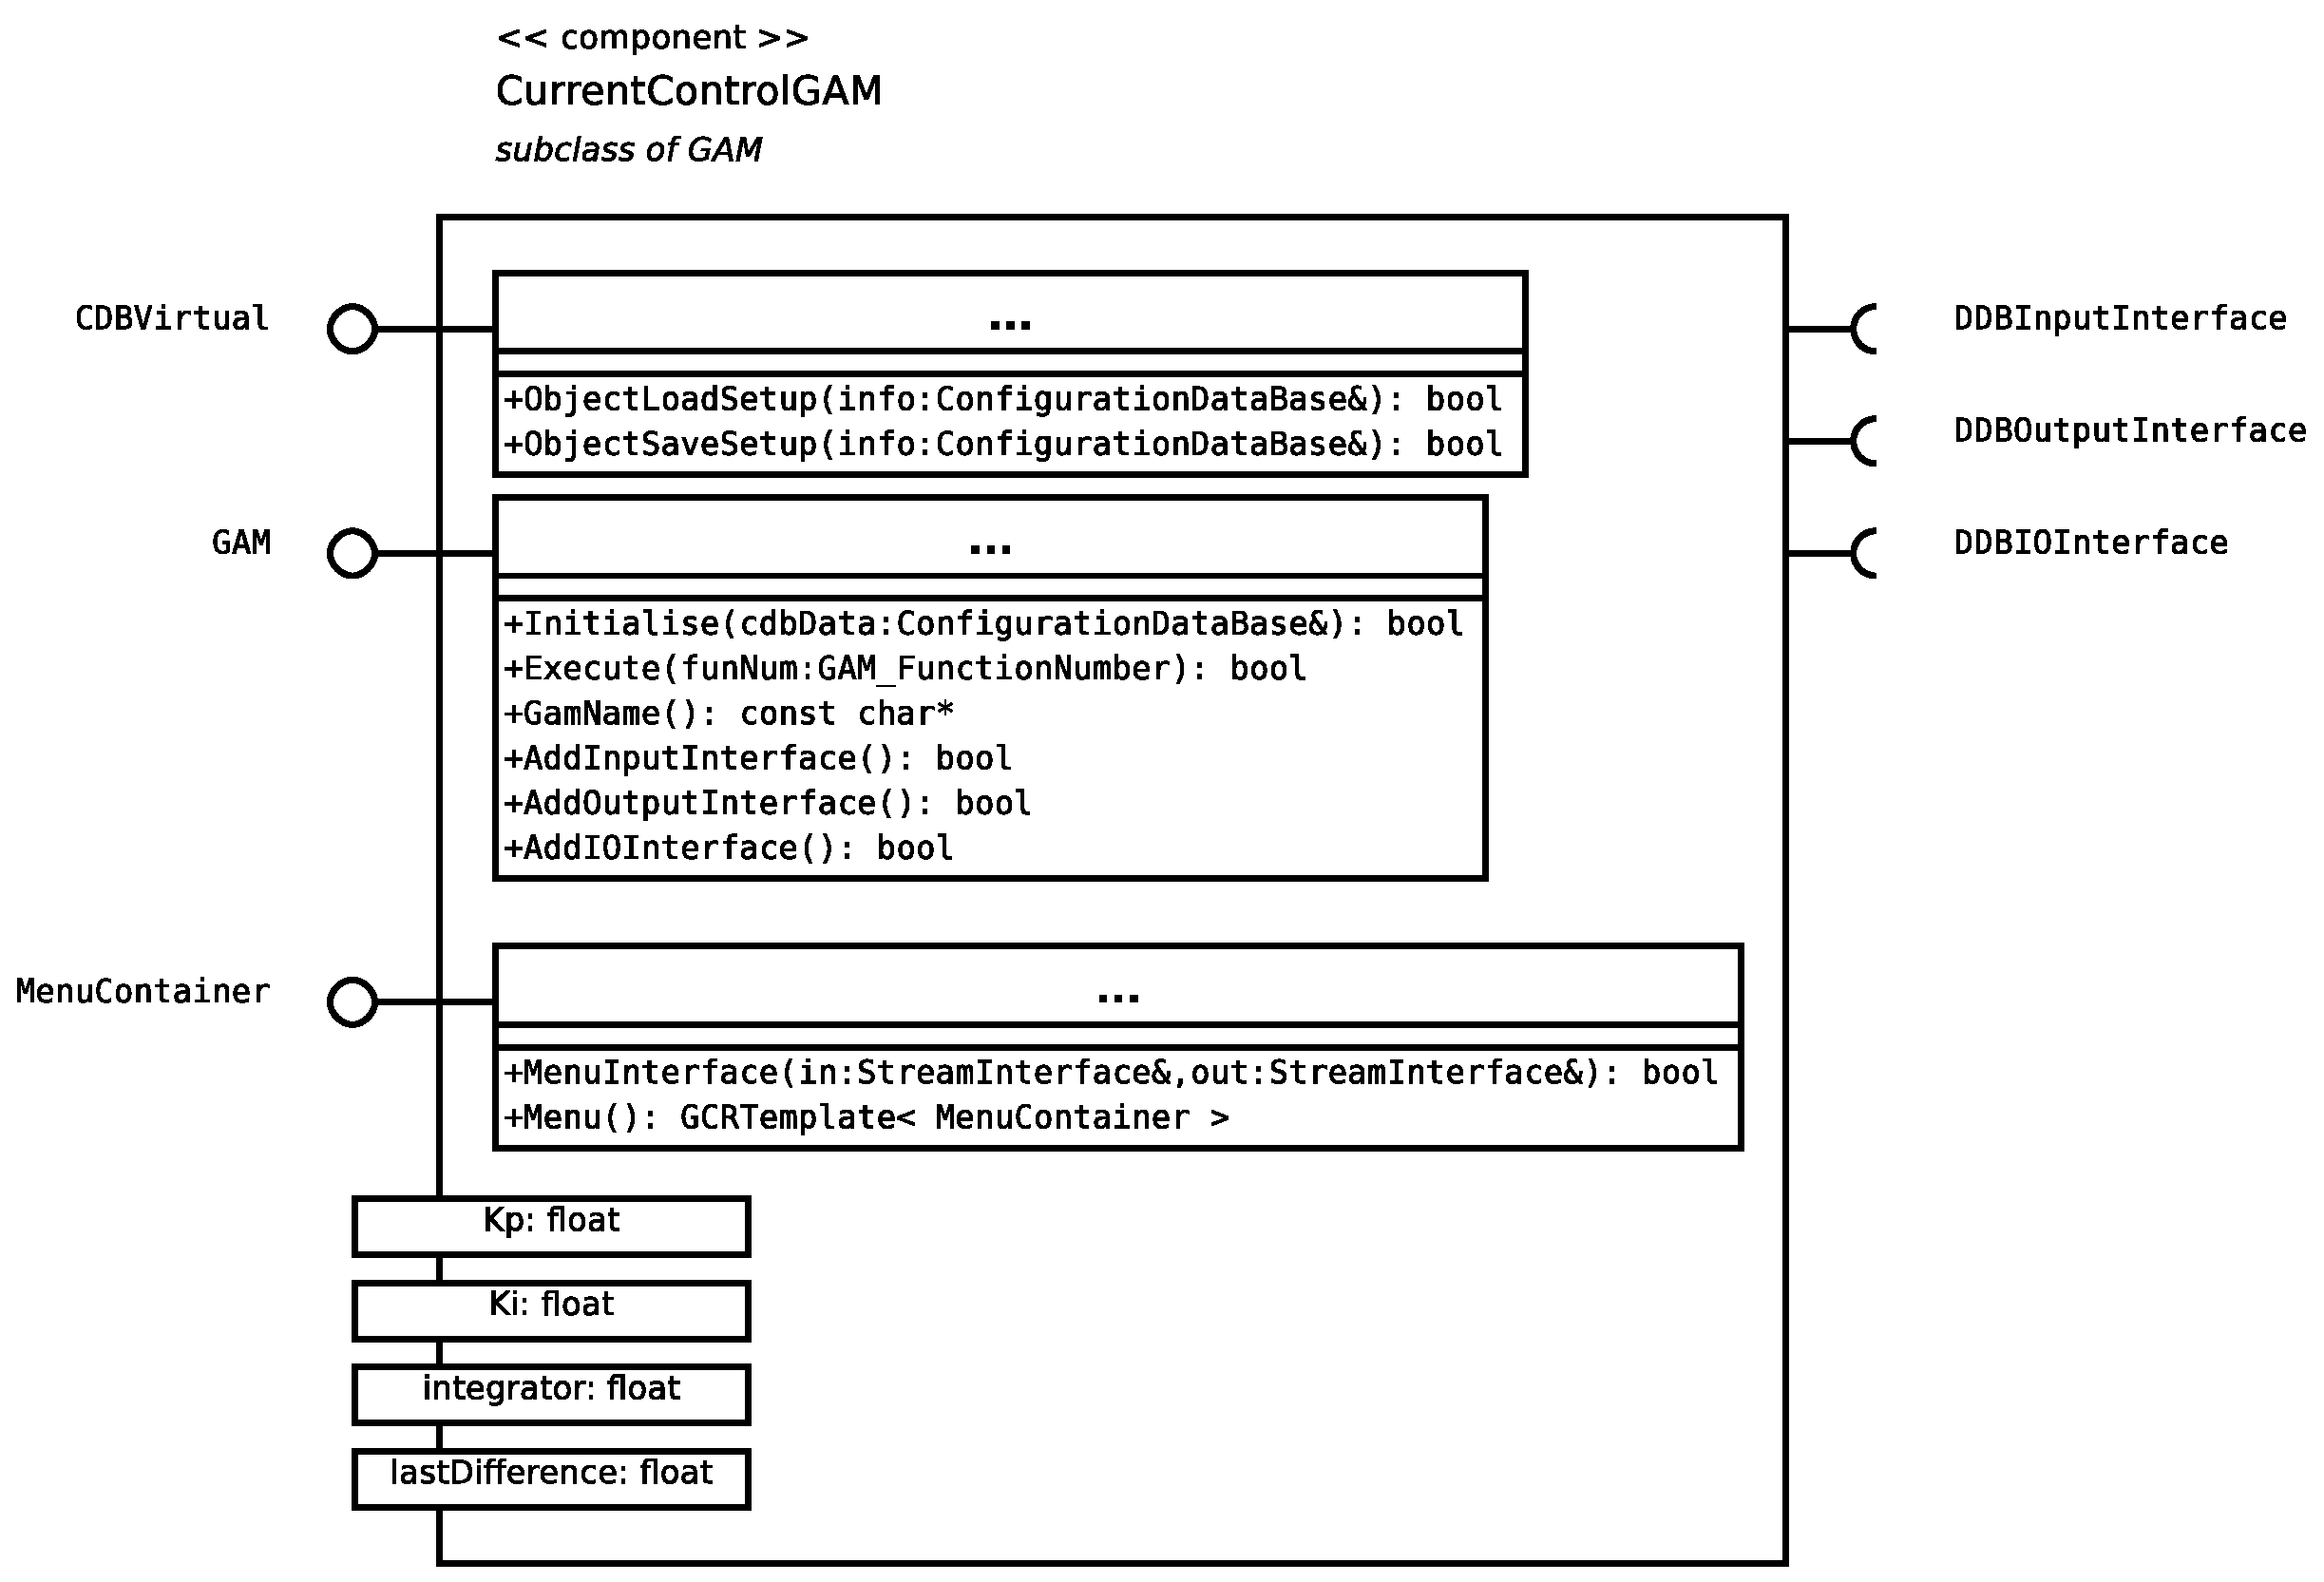
\includegraphics[width=0.5\textwidth]{MARTe/COM-CurrentControlGAM.eps}
  \caption{MARTe \texttt{CurrentControlGAM}, Component Object Model (Microsoft style) schema.}
  \label{f:MARTe:CurrentControlGAM}
 \end{center}
\end{figure}


Last notes about DDB buffers. The format of buffers must be more clear. Mostly of the time a GAM expect an \texttt{DDBInputInterface} where the buffer has as the first argument a time stamp of 32bit and then an array of values; the \texttt{CurrentControlGAM} just differs exepcting a buffer with the following format.
\begin{lstlisting}[
extendedchars=true,%
basicstyle=\fontfamily{pcr}\fontseries{m}\selectfont\footnotesize, %
stepnumber=1,%
numberstyle=\tiny,%
keywordstyle=\footnotesize\tt ,%
language=C++]
typedef struct _InputData{
    int32 usecTime;
    float currentReference;
    float currentMeasured;
}InputData;
\end{lstlisting}


\section{Remarks}
Just to summarize the content of this chapter we propose Figure \ref{f:MARTe:GAM:io} that shows togheter all GAMs presented here and groups it by input/output capability; Figure \ref{f:MARTe:GACQM:io} shows and group GACQM by its input and output capability and highlight the \texttt{TimeInput} characterization.

\begin{figure}[h!]
 \begin{center}
  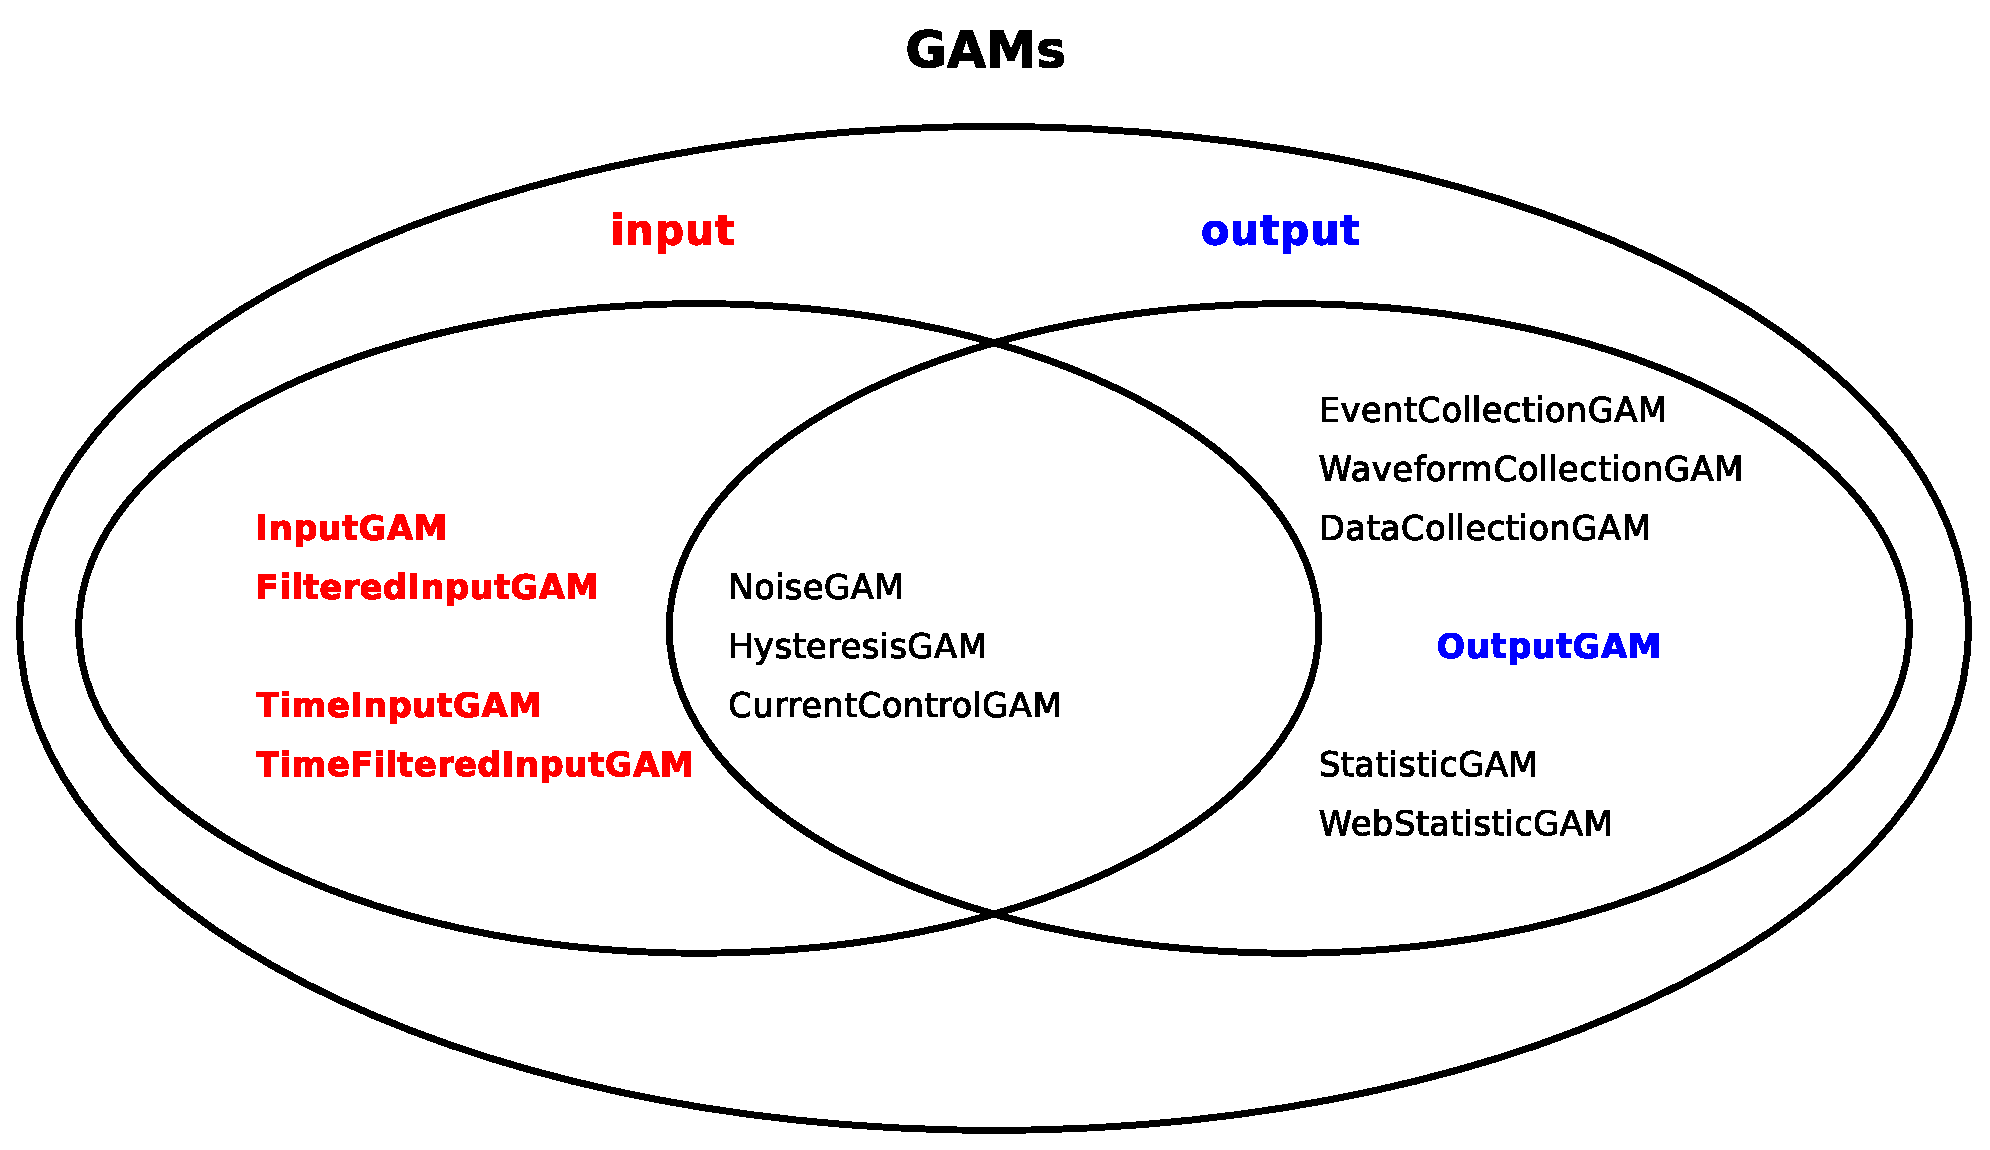
\includegraphics[width=0.66\textwidth]{MARTe/GAMs-io.eps}
  \caption{MARTe GAMs grouped by I/O capability (source/sink of data) concerning the block diagram.}
  \label{f:MARTe:GAM:io}
 \end{center}
\end{figure}

\begin{figure}[h!]
 \begin{center}
  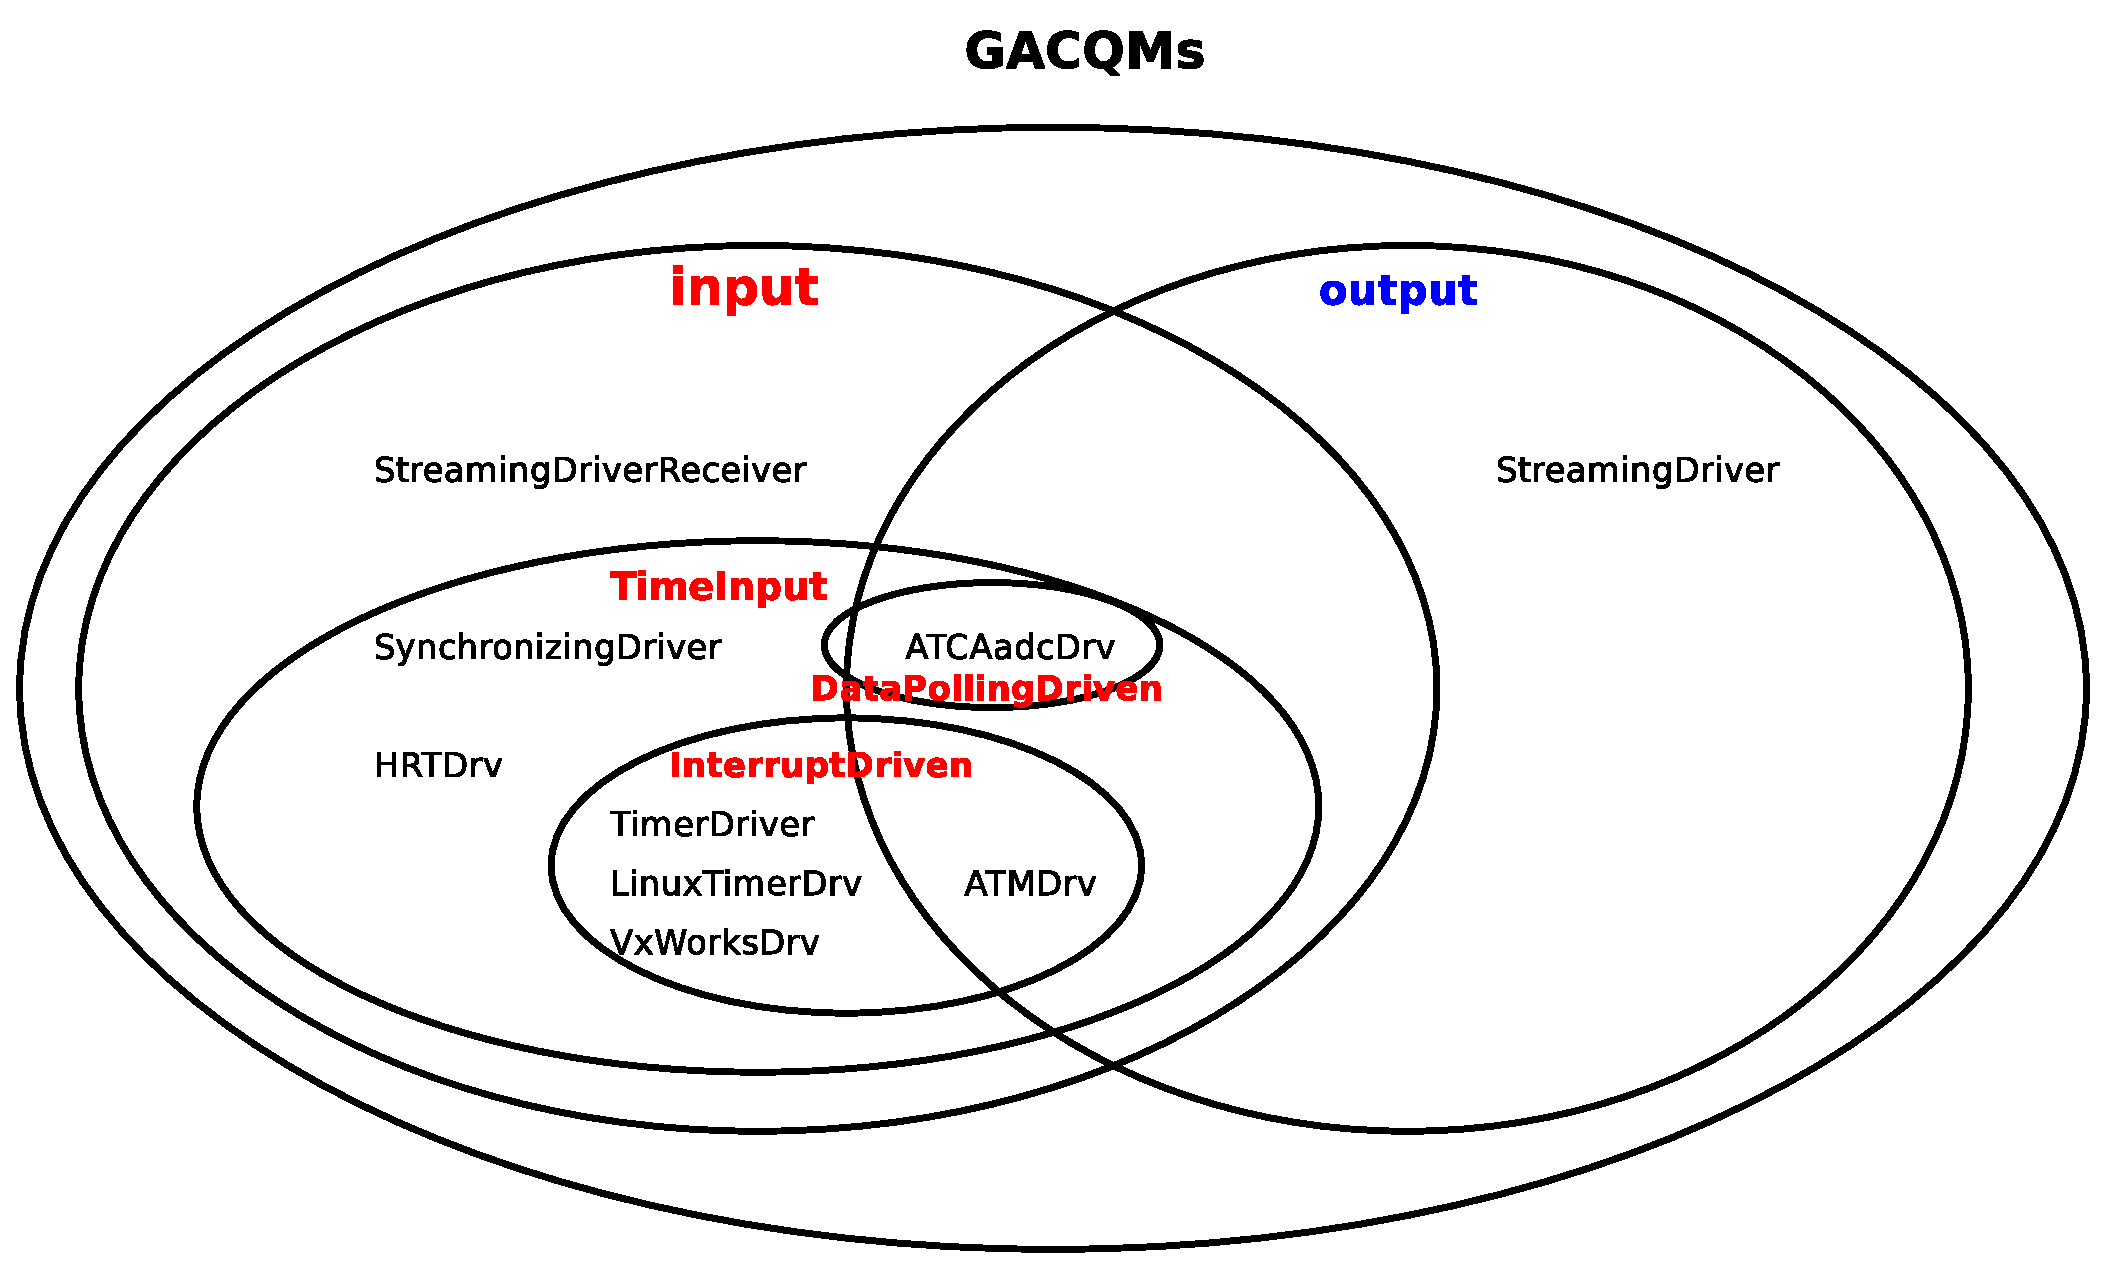
\includegraphics[width=0.66\textwidth]{MARTe/GACQMs-io.eps}
  \caption{MARTe GACQMs grouped by I/O capability (source/sink of data) concerning the environment.}
  \label{f:MARTe:GACQM:io}
 \end{center}
\end{figure}


